%\documentclass[british]{ntnuthesis}
\documentclass[british,titlepage,twoside]{ntnuthesis}
\setlength{\parindent}{0em}
%\renewcommand{\baselinestretch}{1.5} 
\title{Observable Effects of Selected\\ Phasor Measurement Unit\\ Time Delay Attacks}
\shorttitle{Observable Effects of Selected PMU TDAs}
\author{Gustav Oskar Sivertsen}
\shortauthor{Gustav O. Sivertsen}
%\date{CC-BY \ntnuthesisdate}
\date{\today}
%\usepackage[acronym,style=index]{glossaries}
\usepackage{csquotes}
\usepackage{amsmath}
\usepackage{array}
\usepackage{xcolor}

\usepackage[most]{tcolorbox}
\let\includegraphicsold\includegraphics
\renewcommand{\includegraphics}[2][ ]{\tcbox[size=small, standard jigsaw, opacityback=0]{\includegraphicsold[#1]{#2}}}
\usepackage{soul}
%\setglossarystyle{index}
%\usepackage{glossary-mcols}
%\setglossarystyle{index}
%\setglossarystyle{listdotted}
\usepackage{floatflt}
\usepackage{float}
\usepackage{fbox}
\usepackage{setspace}
%\usepackage{natbib}
 \usepackage{tocvsec2}
%\usepackage{caption}
%\usepackage{subcaption}
\makeglossaries
%\addbibresource{thesis-template.bib}
\addbibresource{thesis.bib}
%\usepackage{graphicx} 
\makeatletter
\newbibmacro*{cite:author}{%
  \iffieldequals{namehash}{\cbx@lasthash}
% Multiple cites in one command
   {\setunit{\compcitedelim}%
    \usebibmacro{cite:plabelyear+extrayear}}%
% Single cite
   {\ifthenelse{\ifnameundef{labelname}\OR\iffieldequalstr{entrytype}{patent}}
% No author/editor
     {\usebibmacro{cite:noname}%
%       \setunit{\nameyeardelim}%
%       \usebibmacro{cite:plabelyear+extrayear}%
       \savefield{namehash}{\cbx@lasthash}}
% Normal cite
     {\ifnameundef{shortauthor}
        {\printnames[labelname][-\value{listtotal}]{labelname}}
        {\ifciteseen
          {\printnames{shortauthor}}
          {\printnames[labelname][-\value{listtotal}]{author}\addspace\printnames[sabrackets]{shortauthor}}}
%      \setunit{\nameyeardelim}%
%      \usebibmacro{cite:plabelyear+extrayear}%
      \savefield{namehash}{\cbx@lasthash}}}%
   \setunit{\multicitedelim}}

\DeclareCiteCommand{\citeauthor}
  {\usebibmacro{cite:init}%
   \usebibmacro{prenote}}
  {\usebibmacro{citeindex}%
   \usebibmacro{cite:author}}
  %{}
  %{\usebibmacro{postnote}}https://www.overleaf.com/project/5e2c288573fa800001d123b0

\makeatother





\begin{document}


\setstretch{1.1}

\chapter*{Abstract}

%The \texttt{ntnuthesis} document class is a customised version of the standard \LaTeX{} \texttt{report} document class. It can be used for theses at all levels – bachelor, master and PhD – and is available in English (British and American) and Norwegian (Bokmål and Nynorsk). This document is ment to serve (i) as a description of the document class, (ii) as an example of how to use it, and (iii) as a thesis template.


The traditional electrical power grid, responsible for the supply of electrical power to consumers of electric power, is in the process of being transformed to a network-controlled automated system for supplying electric power to consumers.
As a part of this transformation, the control and monitoring subsystems of the classic power grid is transformed from being a location-based closed system, to a Internet-connected Smart Grid. In addition, network-connected devices measuring and adjusting power consumption, are deployed to the locations of power consumers.
The transition described opens the possibility of the power distribution infrastructure being a victim of malicious Cyber attacks, with the potential intention to cause power grid blackouts, as well as severe damage to critical power grid infrastructure. The topic of my thesis, is to investigate potential effects of exposing phasor measurement units to time delay attacks, by exploiting known vulnerabilities in the IEEE 1588 Precision Time Protocol, observing any consequences such exposure might have on Synchrophasor measurements, as well as attack detectability.
The results obtained indicates a relatively high possibility of getting away with attacks which cold be causing disturbances for grid operation. 


\chapter*{Sammendrag}

Masteroppgaven omhandler sikkerhetstrusler rettet mot smarte nettverk for distribusjon av elektrisk energi. Den tradisjonelle infrastrukturen for distribusjon av elektrisitet  kjennetegnes av sentralstyring og en distribusjon av elektrisistet som ikke er påvirket av abonnentenes faktiske forbruksmønster, men tilpasset estimert behov. Som et svar på de opplevde utfordringer som tradisjonelle distribusjonssystemer har vist seg å ha hatt når det gjelder å sikre en stabilstrøforsyning tilpasset kundenes individuelle behov, har infrastrukturen blitt modernisert. Som en del av moderniseringen, har  infrastrukturen blitt forbundet med Internett, med de utfordringer dette medøfrer relatert til informasjonssikkerhet, med økt fare for driftsavbrugg forårsaket av at ondsinnede aktører utfører tjenestenetkangrap på infrastrukturen. I og med at den moderniserte infrastrukturen har behov for kontinuerlig overvåking av distribusjonssystemet, er kravet til presisjon relatert til å merke hendelser med korrekt tidsstempel avgjørende for å få det korrekte bildet av distribusjonssystemets tilstand. Dersom aktører kan forstyrre mekanismene som beregner tidsstemplene til kritiske distribusjonskomponeneter, får operatørene som overvåker og styrer systemene feil beslitningsgrunnlag, som dermed kan trigge responser basert på feilaktig grunnlag. Tidsstemplene blir beregnet basert på tidsdata hentet fra satelittbaserte tjenester som det amerikanske GPS-systemet. Masteroppgavens tema er i hvilken grad smarte kraftdistribusjonssystemer er sårbare for målrettet modifisering av GPS-signalet slik at feil i tidsberegninger skaper planlagte driftsforstyrrelser.
Som en videreføring av temaet, vil oppgaven deretter fokusere på hvilke muligheter det kan finnes for deteksjon av slike hendelser, med tanke på å hindre at angrepene ikke får sin tilsktede effekt.



\chapter*{Acknowledgments}


I would first like to sincerely thank my supervisor, \textbf{Prof. Stephen D. Wolthusen}, for his invaluable involvement and guidance during the entire duration of my master's thesis project, from the definition of the route for me to take in order to complete the thesis, as  well as on the way to project completion.\\ 

I would also like to express my thanks to my co-supervisor \textbf{Dr. James G. Wright}, for his invaluable support and guidance during the last part of my project. 
%I would also like to thank advisor \textbf{Hilde Bakke} for all her help related to the practical issues concerning my  life as a remote student at NTNU Gj\o vik. \\ 


%In addition, I would like to thank former master student \textbf{Beatrice Giannini} for sharing her thesis with me, during the initial phases of my project. \\



%Finally, I would like to express my sincere apologies to to my family, as well as my colleagues and academic acquaintances, for the unintended test of patience caused by my efforts in order to complete my Master thesis project, while being employed in a full-time position as a operations engineer. 

%\bigskip
%\bigskip
%\bigskip

%\begin{quote}
%“Patience is not the ability to wait, but the ability to keep a good attitude while waiting.”
% - Joyce Meyer
    
%\end{quote}


\listoffigures
\listoftables

 \newacronym{ami}{AMI}{Advanced Metering Infrastructure}
\newacronym{amr}{AMR}{Automated Metering Reading}
\newacronym{ban}{BAN}{Building Area Network}
\newacronym{ci}{CI}{Critical Infrastructure}
\newacronym{cia}{CIA}{Confidentiality, Integrity and Availability}
\newacronym{cii}{CII}{Critical Information Infrastructure}
\newacronym{ckc}{CKC}{CYber Kill Chain}
\newacronym{cpg}{CPG}{Classic Power Grid}
\newacronym{cps}{CPS}{Cyber-Physical System}
\newacronym{crsg}{CRSG}{Cognitive Radio Smart Grid}
\newacronym{ddos}{DDoS}{Distributed Denial of Service}
\newacronym{dg}{DG}{Distributed Generation}
\newacronym{dos}{DoS}{Denial of Service}
\newacronym{dr}{DR}{Demand Response}
\newacronym{dsm}{DSM}{Demand-Side Management}
\newacronym{eci}{ECI}{European Critical Infrastructure}
\newacronym{ems}{EMS}{Energy management System}
\newacronym{epri}{EPRI}{Electric Power Research Institute }
\newacronym{fan}{FAN}{Field Area network}
\newacronym{gps}{GPS}{Global Positioning System}
\newacronym{gnss}{GNSS}{Global Navigation Satellite System}
\newacronym{han}{HAN}{Home Area Network}
\newacronym{ian}{IAN}{Industrial Area Network}
\newacronym{ics}{ICS}{Industrial Control System}
\newacronym{ict}{ICT}{Information and Communication Technology}
\newacronym{lan}{LAN}{Local Area Network}
\newacronym{mitm}{MiTM}{Man in The Mittle}
\newacronym{nan}{NAN}{Neighborhood Area network}
\newacronym{nist}{NIST}{National Institute of Standards and Technology}
\newacronym{ntp}{NTP}{Network Time Protocol}
\newacronym{pdc}{PDC}{Phasor Data Concentrator}
\newacronym{pg}{PG}{Power Grid}
\newacronym{pmu}{PMU}{Phasor Measurement Unit}
\newacronym{ptp}{PTP}{Precision Time Protocol}
\newacronym{scada}{SCADA}{Supervisory Control And Data Acquisition}
\newacronym{sdn}{SDN}{Software Defined Networking}
\newacronym{sg}{SG}{Smart Grid}
\newacronym{sm}{SM}{Smart Meter}
\newacronym{telco}{TELCO}{Telecommunication}
\newacronym{tsa}{TSA}{Time Syncronisation Attack}
\newacronym{tve}{TVE}{Total Vector Error}
\newacronym{wams}{WAMS}{Wide Area Measurement System}
\newacronym{wan}{WAN}{Wide Area network}
\newacronym{wsn}{WSN}{Wireless Sensor Networks}

%\glsnogroupskiptrue 
%\printglossary[type=\acronymtype]

\printglossary[type=\acronymtype]

 \tableofcontents

%\lstlistoflistings


\chapter{Introduction and Scope} 

%[Introduction:] The introduction would serve the same purpose as for a smaller research project described in \cref{sec:development}, but would normally be somewhat more extensive. The \emph{agenda} part should inform the reader about the structure of the rest of the document, since this may vary significantly between theses.

During the last few centuries, the society  has become increasingly dependant on access to a stable and reliant supply of electrical power. The usage of electrical power in order to provide heating, lighting, as well as running various electrical appliances, like washing machines and wireless access points, has created an increased demand for electricity. The increased demand for electricity has transformed the classical \acrfull{pg} infrastructure, initially consisting of local electricity distribution infrastructure,  into a nation-wide power distribution infrastructure network, known as the \acrfull{sg}.







\section{Background}
As described in \cite{BlumeStevenW2007Epsb}, electricity is supplied by the Power Grid infrastructure, consisting of power generating facilities,\footnote{like hydro-based facilities utilising water to generate electricity, or nuclear power plants.} and transmitted via a high voltage transmission infrastructure, before being converted to  lower voltage electrical currents, fed to the distribution infrastructure for distribution to paying consumers.


The classic \acrlong{pg} was under manual and centralised control, and monitored through a centralised and unidirectional \acrfull{scada} system.
The progressively increasing dependency on a reliable supply of electrical power makes it vital to avoid power outages, which will result in reduced temperature in buildings lacking alternative sources of heating, as well as the absence of vital services, like electronic payments, telecommunications, and transportation.
%As described in \cite{rehmani2019software}, the traditional \acrlong{pg} has proven to be unable to meet the demands of the future for a flexible and reliable power distribution system.
Therefore, several organisations, like the \acrfull{nist} and the \acrfull{ieee}\footnote{amongst others.} has made considerable efforts in order to produce standards, in order to define the \acrlong{sg}.


\subsection{The conversion of the Power Grid to the Smart Grid.}



%As described in \cite{greer2014nist} and  \cite{MRABET2018469}, the  \acrlong{sg} consists of seven domains, defined as presented in table \ref{tab:SmartGRID-Roles-of-domains}

In order to address the future demands for electrical power, the uni-directional control mechanisms of the traditional power grid is replaced by the bidirectional flow of information characteristic of the modern \acrshort{sg}. The control mechanisms of the modern \acrshort{sg} infrastructure is utilising standardised computer networking technology for bidrectional communication.  In order to meet the new requirements for monitoring, the \acrshort{pg} is connected to the Internet. 
The authors of \cite{colak2020effects}  describes the transition from the classical power grid to the smart grid as unavoidable.
%The \acrfull{sg} is the modern improvement of the classical \acrfull{pg}, meeting the increased demand for a more reliable, stable and flexible power distribution infrastructure.

For the system to meet the \acrlong{sg} monitoring  and control capability requirements, the \acrfull{wams} has been implemented. 
A number of \acrlong{pmu}s are connected to a \acrlong{pdc}, which transmits synchronised phasors to the \acrshort{wams} Control Center. The usage of the resulting synchrophasors enables the \acrshort{sg} operators to get a more fine-grained view of the operational state of the \acrshort{sg}, than obtainable by a classic \acrshort{scada} system. As part of a modern \acrshort{wams} system, \acrfull{se} algorithms has been developed, in order to counter cyber attacks or unintentional \acrshort{pg} failures. In addition to the \acrshort{se} algorithms, several security enhancements to relevant \acrshort{sg} protocols are being implemented in an attempt to reduce the attack surface available to potential threat actors.







\subsection{Security vulnerabilities of the Smart Grid WAMS}
As a consequence of the \acrlong{sg} infrastructure being connected to the Internet, the infrastructure is becoming vulnerable to cyber attacks.   The \acrlong{sg} \acrlong{wams} is the main control system of the \acrshort{sg} and, as such, constitutes a complex system vulnerable to numerous cyber attacks, as identified by several papers,  like for instance \cite{li2019review} and  \cite{kateb2018enhancing}.

The modern interconnected \acrshort{sg}, featuring a \acrshort{wams} system receiving an increasing number of synchronised phasors,\footnote{Phasors are synchronised at \acrshort{pmu}s, before being transferred via \acrshort{pdc}s to the WAMS,}  is increasingly dependant on synchronised time.
%As explained by \cite{xue2021data}, a \acrlong{tsa} might be successfully completed without prior knowledge of the infrastructure being targeted. \\ 
%Given the vulnerability of the \acrshort{gnss} to \acrshort{tsa}, the ever increasing likelihood of one or more of the \acrshort{pmu}s of the \acrshort{sg} \acrshort{wams} being the target of a \acrshort{tsa} causing any kind of havoc to the grid, makes this topic vital for further studies.
In \cite{ullmann2009delay}, several types of cyber attacks are identified. Most of the attacks described by \citeauthor{ullmann2009delay}in \cite{ullmann2009delay}, with the exception of the "Delay of synchronization messages" attack are, to some extent, being mitigated by various means. The 
Delay  synchronization messages attack however, may\footnote{if performed by a sophisticated threat actor having sufficient knowledge of valid traffic patterns.} prove to be a stealthy attack, thereby avoiding detection.  The aim of these sophisticated threat actors would, therefore, be to stay undetected, while creating a substantial amount of disturbance to the operation of the \acrshort{sg}. \\ 
% Given the aforementioned tendency of going online with components essential to the proper control of the \acrshort{sg}, opens the possibilities for attackers to  interfere with, for instance,  unencrypted synchrophasor data transmission from \acrlong{pmu}s to their corresponding \acrlong{pdc}s, by exposing them to a \acrlong{mitm} attack.
%A presentation of various attack strategies are given by \citeauthor{li2019review} in \cite{li2019review}, as well as by \citeauthor{paudel2017attack}in \cite{paudel2017attack}.
%The scope of my master thesis, will be to investigate vulnerabilities of \acrfull{tsa}, targeting the \acrfull{wams} in order to disturb proper \acrshort{sg} operation.
%The scope of my master thesis, will be to investigate vulnerabilities of the synchrophasor protocols, targeting the \acrfull{wams} in order to disturb proper \acrshort{sg} operation.
My thesis will be focusing on time delay attacks against \acrshort{pmu}s, and investigate which effects a number of selected delay attacks may have on the \acrshort{pmu} output, as visualised by a simulation. 


\section{Definition of scope}

%The introduction of Synchrophasors have enabled the \acrshort{sg} operators to gain increased\footnote{as compared to the traditional SCADA system} control over the operational state of the modern \acrlong{pg}. 
%As described by  \cite{ullmann2009delay}, the standardisation of Synchrophasor data transmissions will, with the introduction of transmission encryption, impose increasingly higher levels of security to the \acrlong{sg}. 
%As further described by \cite{ullmann2009delay}, the \acrlong{tda} still remains a threat to the \acrlong{ptp}.% which, according to \cite{bishop2022iec}, is identified as the preferred standard to be used for Time Synchronisation  for \acrshort{sg}s operating according to the IEC 61850 standard.


As \citeauthor{moussa2016security}denotes in TABLE II of \cite[p. 1959]{moussa2016security}, the paper \cite{ullmann2009delay}\footnote{ The paper, entitled "Delay attacks — Implication on NTP and PTP Time Synchronization",\\ is  identifiable as reference [13] in \cite{moussa2016security}.} by \citeauthor{ullmann2009delay}, is lacking experimental verification of the attack, the countermeasures  
suggested, \textit{as well as any effects of the \acrshort{ptp} delay attack}. 

%On the other hand, the quantitative study of \cite{ullmann2009delay}, is evaluating the consequences of the \acrshort{ptp} delay attack.\footnote{ as identified by the \textbf{Advantage} column of \textbf{TABLE II} of \cite[p. 1959]{moussa2016security}. }\\ 
Given the unresolved \acrshort{tda} vulnerability of the \acrshort{ptp}, in addition to the absence of a description of any effects of the attack, identified by \cite{moussa2016security} as a disadvantage of \cite{ullmann2009delay}, my contribution will, specifically, be to investigate possible effects of exposing a \acrlong{pmu} to a \acrlong{tda}. 
%The simulation is performed by producing a new signal by shifting the original signal by a number of steps, according to the formula $y(timeStamp)= x(timeStamp + delay)$.
%Given an attack stealthiness requirement, which delay level produces a result within the graph signal similarity tolerance level specified?
%In order to limit the scope of my investigation, two categories of attacks are specified:
%\begin{enumerate}
%    \item An attack by which the delay level is 0 before the attack, and increasing instantly to the specified level is reached.
%    \item An attack by which the delay level is 0 before the attack, and increasing one sample each second until the specified level. 
%    
%\end{enumerate}
%In each case, the attack is initiated at a specified sample time, and terminated at a specified time during the time span of the simulation. The termination of a real Time Delay attack could be intentional\footnote{Like the simulated controlled attack termination initiated by the threat actor}, or caused by a genuine synchronisation of the PTP clock under attack.
\section{Research questions}
The main goal of my project, is thus to investigate which potential effects a selection of \acrlong{tda}s might have on \acrshort{pmu} output. 

In order to proceed with the \acrlong{tda} vulnerability investigation, I have selected the following research questions:

\begin{enumerate}
    \item Which effects of the time delay attack simulations covered by this study, is observable on the visualised output of the PMU simulated?
    \item For a selected similarity requirement, what delay level could be observed as being within similarity tolerance levels?
    \item Which of the delay functions covered would be preferred, in order for the malicious threat actor to stay undetected?    

    %\item How might a \acrshort{sp} attack be mitigated?
    %\item Investigate the GPS spoofing vulnerability of the \acrshort{sg} monitoring and control system.
    %\item Investigate GPS Spoofing detection and mitigation techniques. 
    %\item Investigate how \acrfull{sdn} might be applicable to improve \acrshort{sg} Security
    %\item Investigate SDN-based SG \acrshort{dos} detection and mitigation potentials. 
    %\item 
\end{enumerate}

In order to investigate the topic further, I will conduct a theoretical study of relevant concepts, before performing a number of experiments before discussing the results presented, with the aim of being able to conclude on possible answers to the research questions. 



\section{Outline of the rest of the thesis}

%Following the introductory study of the concept of the \acrshort{sg}, I will study relevant protocols, before investigating the nature of a number of  time delay attacks.


This introductory chapter is followed by a theoretical part, consisting of a chapter introducing the (smart) power grid, followed by chapters covering topics like the \acrshort{wams} control system, \acrfull{sg} power flows status monitoring, and \acrlong{sg} cyber attacks and threat actors. 
%A chapter on \acrlong{sg} security, follows, including a cyber security vulnerability assessments of the \acrshort{sg}. As the main focus will be on \acrshort{sp} attack vulnerabilities, the \acrshort{sg} Control System, as well as the dependability of correct Time Synchronisation data, and finally time synchronisation attack vulnerabilities, are covered. 
%In order to investigate the \acrshort{sp} attack  vulnerabilities of the \acrlong{sg}, a chapter presenting aa number of \acrshort{sp}s, covering ther vulnerabilities,   attack detection and mitigation techniques follows the chapter on \acrshort{sg} security.
%The chapter on TSA detection and mitigation techniques is 
The remaining chapters covers the experimental investigation of the \acrlong{tda} on \acrlong{pmu} output. The methodology chapter includes a detailed description of the model implementation and usage, before a number of experiments are presented and described in detail.
My thesis is finalised by the inclusion of a chapter presenting results, before the discussion and conclusion chapters, including the suggestions for further work, at the end of the thesis. 
%\begin{itemize}
%    \item A description of the various parts of the architecture of the \acrshort{sg}.
 %   \item A presentation of a selection of previous vulnerability assessments of the \acrshort{sg} related to the confidentiality, integrity, availability and accountability of the \acrshort{sg}, in order to identify any vulnerabilities related to  denial of service attacks.
 %   \item A presentation of a selection of previous studies related to utilising \acrshort{sdn}  in order to reduce the risk of  \acrshort{sg}  \acrshort{dos} attacks.
%\end{itemize}

%\begin{itemize}
    %\item Provide an overview of \acrshort{sg} \acrshort{dos} vulnerabilities.
  %  \item Provide an overview of possible detection and mitigation techniques.
 %   \item Complete experiments in order to evaluate selected mitigation techniques.
%\end{itemize}

 



\chapter{The power grid}
%\section{History of the power grid}
%conventional power Grid






\section{The Conventional Power Grid}
The \acrfull{cpg} is described in several papers, and books like \cite{BlumeStevenW2007Epsb}, as  a uni-directional, manually controlled, power distribution system.  

\begin{figure}[ht]
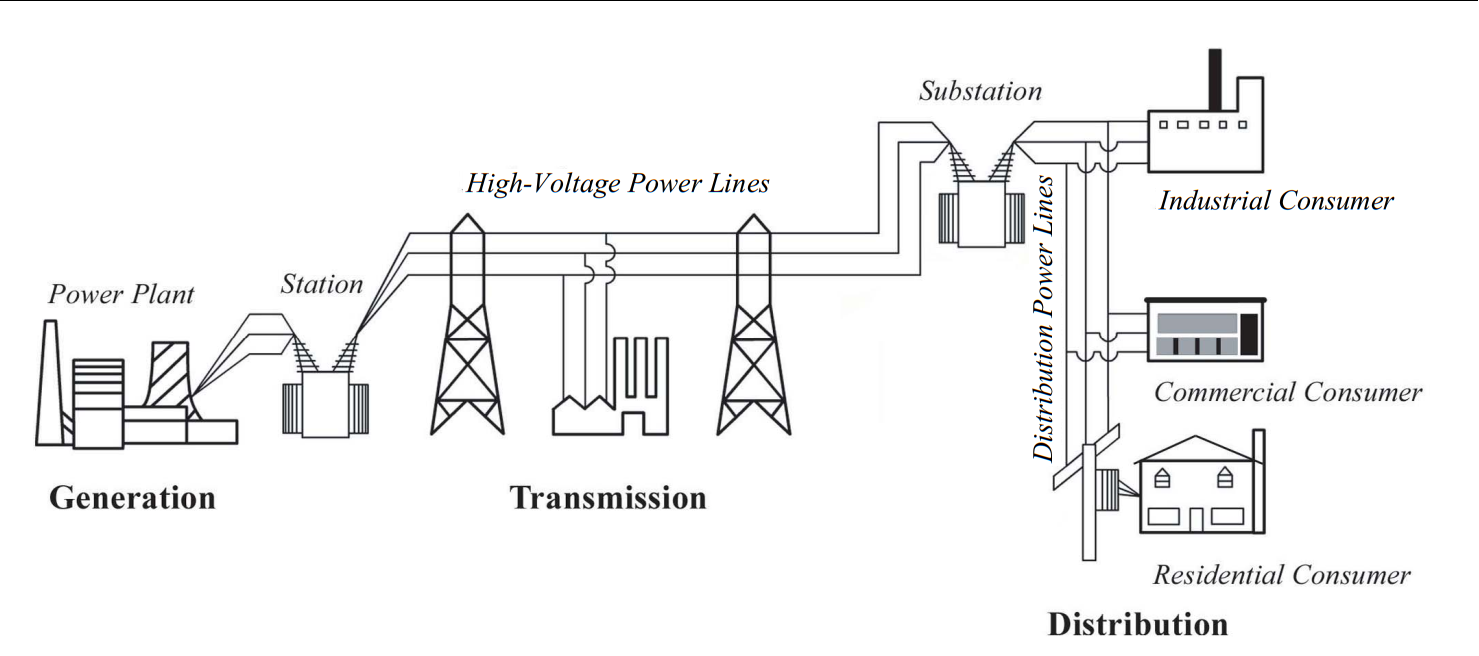
\includegraphics[width=\linewidth]{figures/Blume-PowerGrid-SystemOverView.png}
\caption[Power Grid System Overview]{Power Grid System Overview , as presented in \cite{BlumeStevenW2007Epsb}}
\label{fig:Blume-PowerGrid-SystemOverView}
\end{figure}



\subsection{Overview of the Conventional Power Grid}
The \acrlong{cpg} is a system by which electric power is centrally generated, transmitted, and distributed to industrial, residential,and commercial end users, in order to ensure a reliable access to a sufficient amount of electrical energy. 
\newpage
The \acrlong{cpg}, as described in \cite{BlumeStevenW2007Epsb}, consists of the following subsystems:

\begin{itemize}

 \item The \textbf{Generation Subsystem} which Generates electric power from various sources of energy, to be transmitted for distribution to Consumers. Some examples of installations generating electrical power are nuclear power plants, as well as hydroelectric power plants, feeding water-driven turbines in order to generate power.
 \item The \textbf{Transmission Subsystem} which transmits electric power from the Generation subsystem to the Distribution Subsystem. The current is transmitted via high voltage power lines, minimising energy loss over longer distances.
 \item The \textbf{Distribution Subsystem} which distributes electric power to end users, after converting the high voltage input into lower voltage levels, suitable for consumption.
 \end{itemize}

As described in Chapter 2.3 of \cite{Rihan2018} %\cite{SmartGridOverview2013}
, the \acrlong{cpg} is facing challenges, related to Black Outs adhering to the increased demands for electrical power . 


%\section{The Smart Grid}
%smart Grid
\section{The Smart Grid}




In order to provide a description of the \acrfull{sg}, a description of the characteristics of the \acrlong{cpg} is provided.





As described in  \cite{BlumeStevenW2007Epsb} by \citeauthor{BlumeStevenW2007Epsb}, some of the characteristics of the \acrlong{cpg} are:

\begin{itemize}
\item Power is generated in real time. In the event a consumer is "flipping a power switch," the power grid must have sufficient resources in order to keep the voltage levels at an acceptable level.
\item The \acrlong{cpg} is controlled by a central management facility known as the \acrfull{scada} subsystem. The monitoring and management of the \acrshort{pg} is initiated from the Control Center, utilising unidirectional communication channels. 
\item The \acrlong{cpg} \acrlong{scada} subsystem is offline, i. e. not connected to any publicly available network. Therefore, operational duties must be performed by personnel physically located at dedicated operational sites.

\end{itemize}

The \acrlong{cpg} originates from the local society-serving power generation facilities initiating the supply of electrical power, which over the years were interconnected to form a grid, connecting consumers to a network of several power generating facilities, providing a more flexible power distribution infrastructure. 


\subsection{Overview of The Smart Grid}


The \acrfull{nist} has published a \hl{conceptual} model of the smart grid, as shown in 
figure \ref{fig:NIST-SmartGRID-ConceptualModel}.



\begin{figure}[ht]
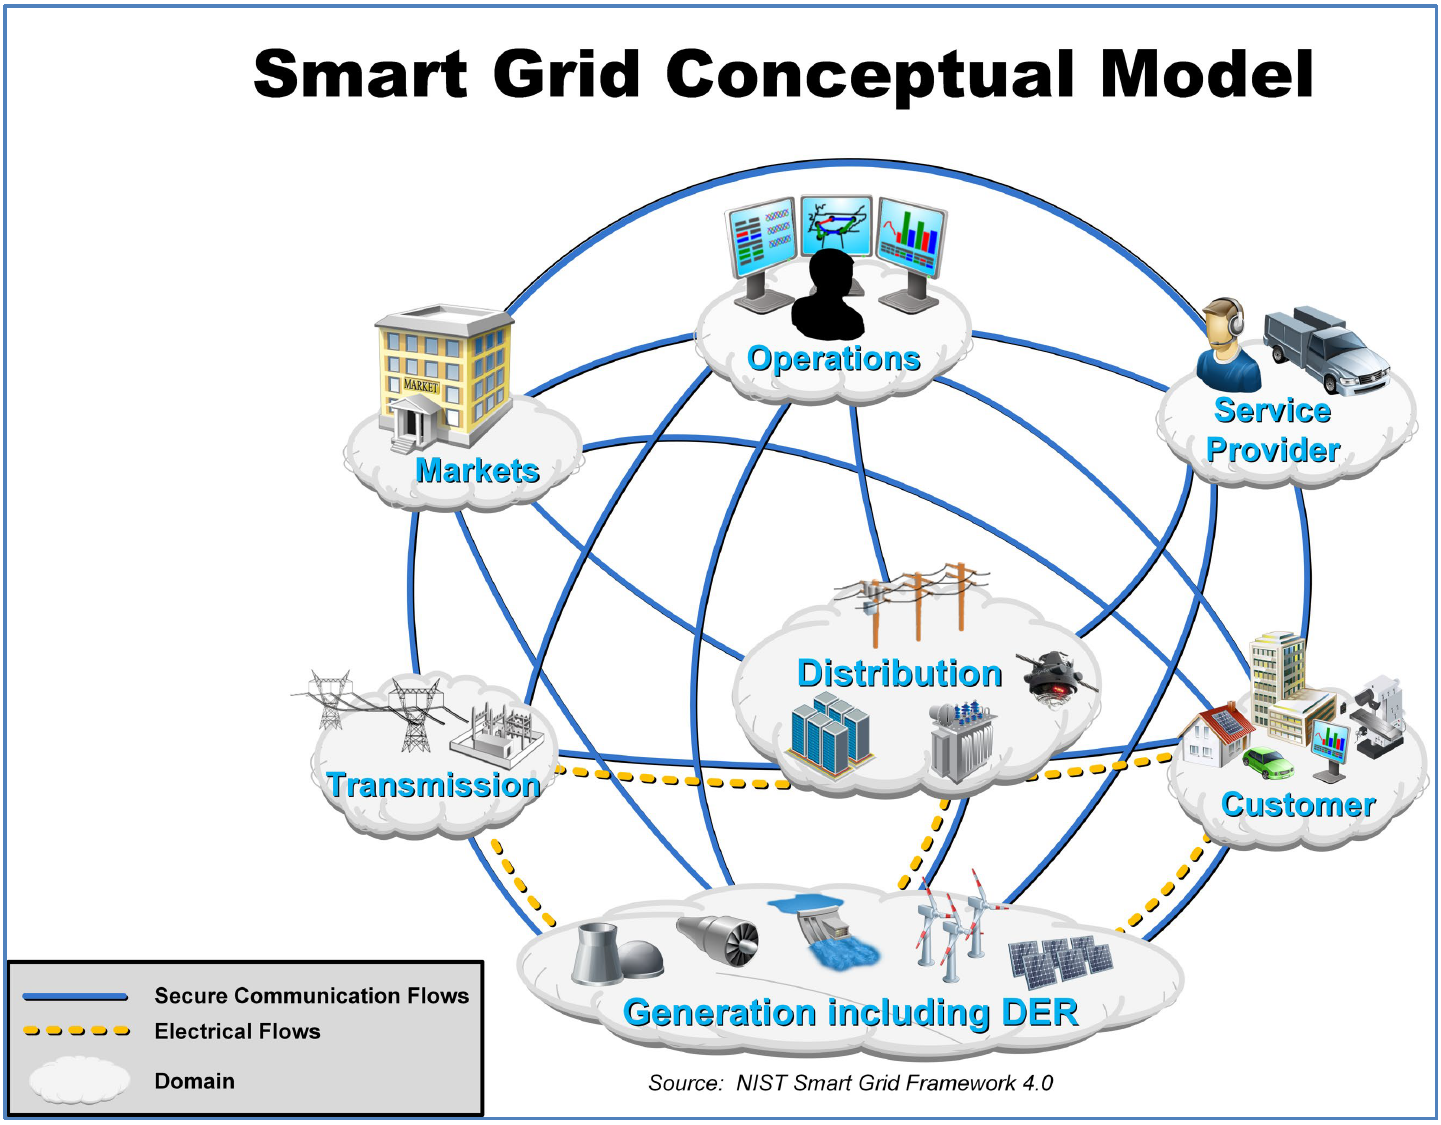
\includegraphics[width=\linewidth]{figures/NIST-SmartGRID-ConceptualModel.png}
\caption[Smart Grid Conceptual Model]{Updated \acrlong{sg} conceptual model, as presented in \cite[p. 13]{gopstein2021nist}, Figure 4}
\label{fig:NIST-SmartGRID-ConceptualModel}
\end{figure}






The \acrlong{sg} adds Information and Communication Technology (ICT) to the \acrlong{cpg}, in order to transform the  unidirectional communication lines of the monitoring and control infrastructure of the \acrlong{cpg}, into an infrastructure utilising two-way communication between the various parts of the \acrlong{sg} infrastructure. 






%\subsection{The Smart Grid: Critical Information Infrastructure}
%According to \cite[p. 610]{Bîrleanu2019}, the \acrlong{sg} consists of the following subsystems:

%\begin{itemize}
%\item \textbf{the conventional  power grid}
%\item \textbf{intelligent equipment} 
%\item \textbf{communication infrastructure}
%\end{itemize}

%\cite{Bompard2012}...

%...\acrlong{sg} Subsystems
%\begin{itemize}
%\item 
%\end{itemize}




\subsection{The Smart Grid Domains}




The \acrshort{sg} consists of seven domains, as shown in \figureautorefname { }\ref{fig:NIST-SmartGRID-ConceptualModel}:


    \subsubsection{Customer Domain} The customers are the Consumers of Electricity.
    The power infrastructure of commercial or private customers includes \acrfull{ami}, monitoring the amount of energy consumed, both for billing and \acrfull{dr} purposes. Consumers may plan their consumption, avoiding high-cost periods of heavy load, by  selecting time frames of low prices.
    \subsubsection{Markets Domain} The participants of the Markets Domain aims to balance the consumption and demand of electricity, by adjusting prices on electricity. Price adjustments may be used in order to shift consumption from periods of high demand, to periods of low demand.     
    \subsubsection{Service Provider Domain} Services to the Customers,  as well as the Markets and Operators domain, are provided by the Service Provider Domain, fulfilling duties like customer management and billing, as well as a number of emerging services as required. 
    \subsubsection{Operations Domain} This domain consists of Electricity service operators, ensuring efficient and fail-safe \acrfull{sg} operation, by utilising \acrshort{scada} systems and \acrlong{ems}s in order to monitor and control system operational state.  
    \subsubsection{Bulk Generation Domain} The facilities for producing electricity, resides in this domain. In addition to the connection and interaction with  to the Transmission domain, it interacts with the Markets domain, as well as the operations domain.  
    \subsubsection{Transmission Domain} The actors of the Transmission domain aims to reduce energy loss while transmitting a stable and reliable stream of energy from operators in the bulk generation domain to the distribution domain. The market domain provides input on expected level of demand which may require adjustments of the amount of electricity distributed, controlled and monitored by actors in the operation domain.  
    \subsubsection{Distribution Domain} The actors of the Distribution Domain delivers the electricity to consumers according to demand and availability, and monitors generation and consumption data. Bi-directional power-flow is supported. In the case customers have private  power producing facilities, like solar cells and wind turbines, any surplus electricity might be sold, and distributed to other customers.



The authors of \cite{uslar2019applying}, \citeauthor{uslar2019applying} describes an alternative model for the \acrshort{sg}, originating from , and visualised in figure \ref{fig:SGAM}. The model consists of three dimensions, named "Domains", "Zones", and the "Interoperability dimension". 

\begin{figure}[ht]
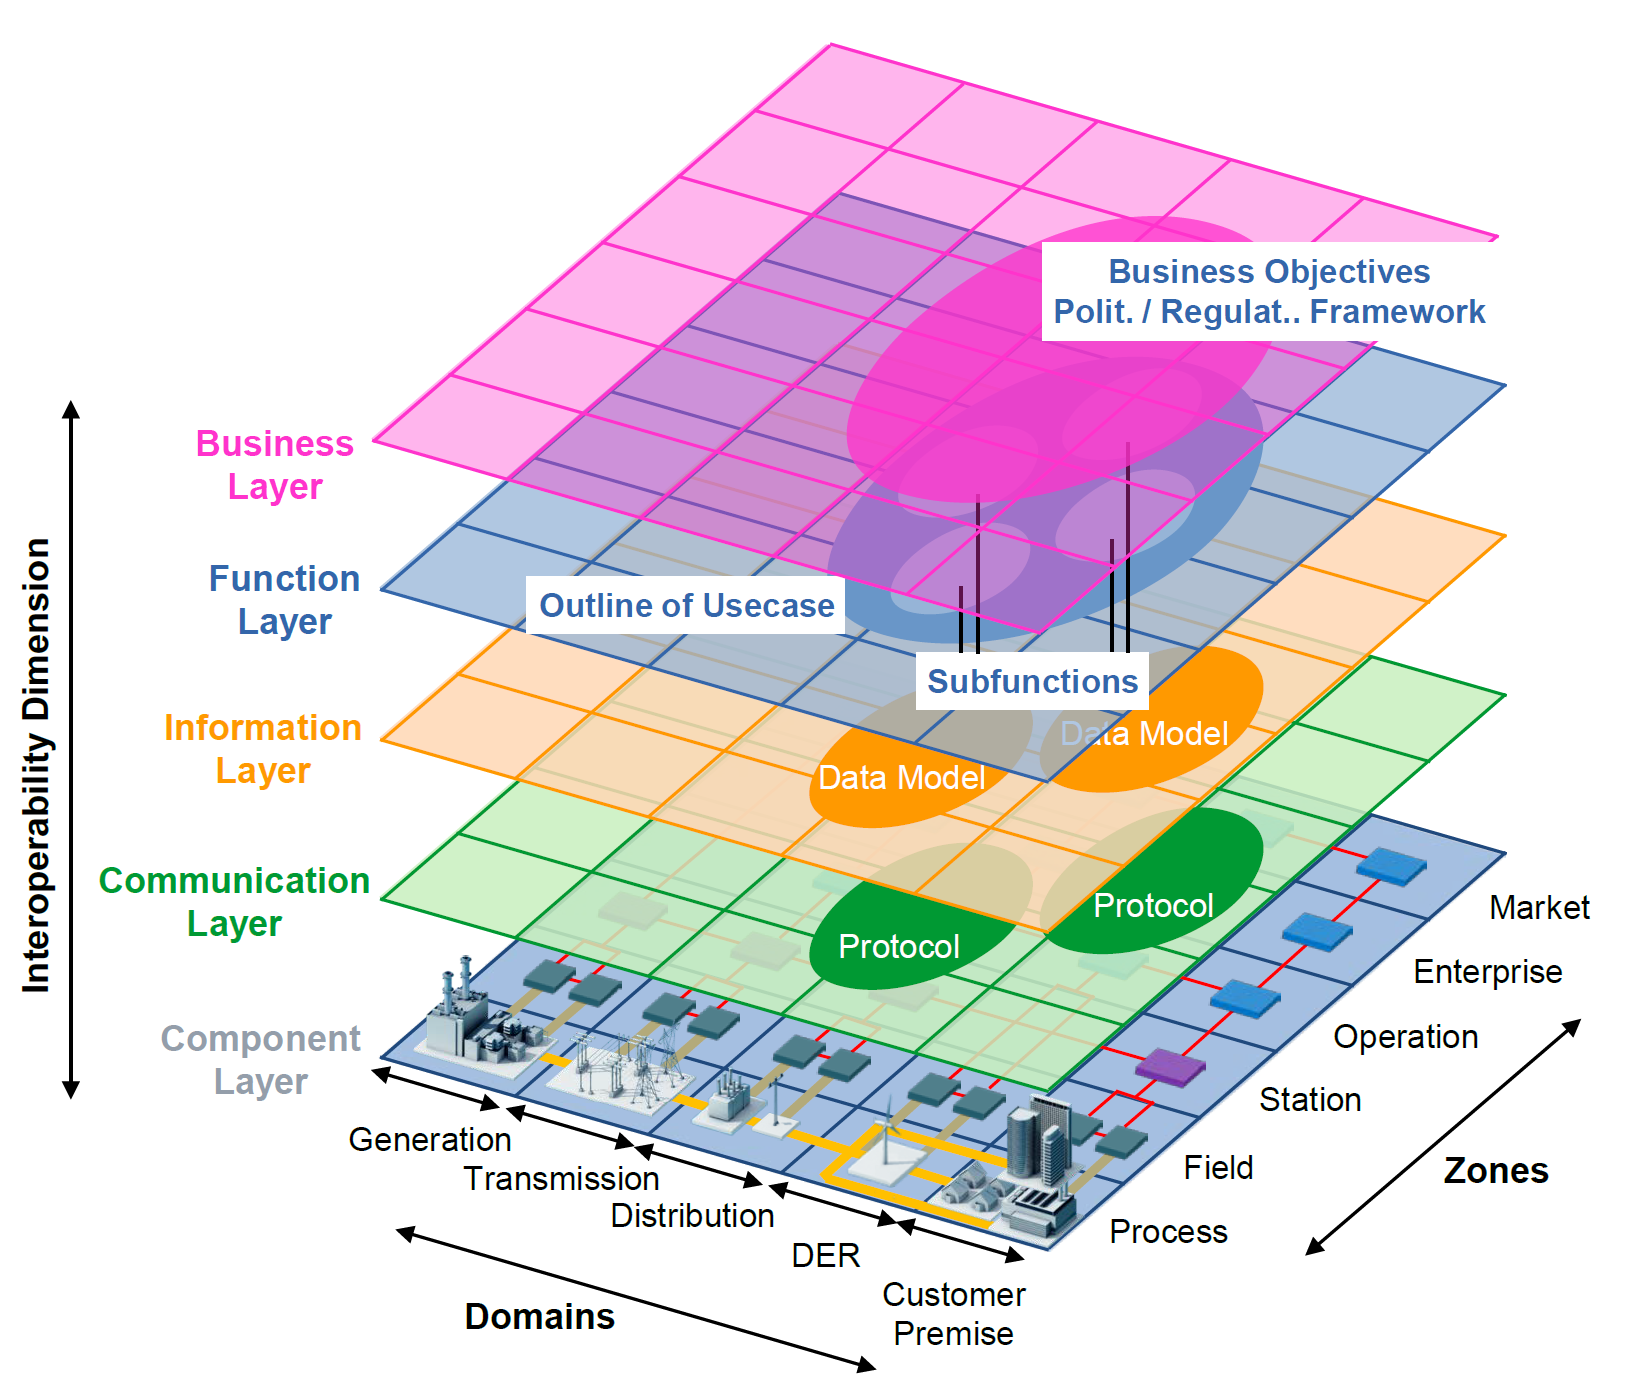
\includegraphics[width=\textwidth]{figures/SGAM.png}
\caption[SGAM Smart Grid Model]{SGAM Smart Grid Model , as presented in \cite{uslar2019applying}}
\label{fig:SGAM}
\end{figure}

The "Domains" dimension consists of the following domains:

\begin{itemize}
    \item The \textbf{Generation} domain:
    \item The \textbf{Transmission} domain:
    \item The \textbf{Distribution} domain:
    \item The \textbf{DER} domain:
    \item The \textbf{Customer Premise} domain:
\end{itemize}




\section{Protocols}
A large number of protocols are defined, in order to standardise the operation of the \acrlong{sg}.

A small selection of these, relevant for the scope of the thesis, are described underneath.

\cite{2021arXiv210311657E} \hl{describes communication protocols} in the  \acrshort{sg}.





The \acrshort{sg} consists of a vast number of both conventional and modern, more dynamic, production facilities, which requires thorough monitoring in order to ensure the optimal distribution of electrical energy. The requirement of a consistently stable and reliable supply of energy is constant, while the amount of energy demanded is dynamically changing according to the demand for power at any time. \\ 

Therefore, the proper \acrshort{sg} operation might be considered virtually impossible without a  close monitoring of current power flow, as well as the ability to instantly adjust the supply of power according to present needs,  without the risk of causing power surges or blackouts. For this purpose, the Wide Area Monitoring System analyses the levels of electrical power as monitored by sensors, synchronised according to a common GPS-controlled time source. \\ 

The correctness of this time source is critical to the reliability, and therefore, the proper operation of the monitoring system, constituting the primary decision criteria for actions controlling the supply of power.



\chapter{The Power Grid Control System}
%Control system
\section{The Conventional Power grid control system}
%- SCADA (historical)

%\subsection{The Classic SCADA subsystem}

The \acrshort{scada} system constituted the core part of the control center of the classic \acrlong{pg}, utilising one-directional communication lines in order to manually control and monitor the operational state of the power grid.

Figure \ref{fig:Blume-SCADA-system} shows the main components of the SCADA system.

\begin{figure}[ht]
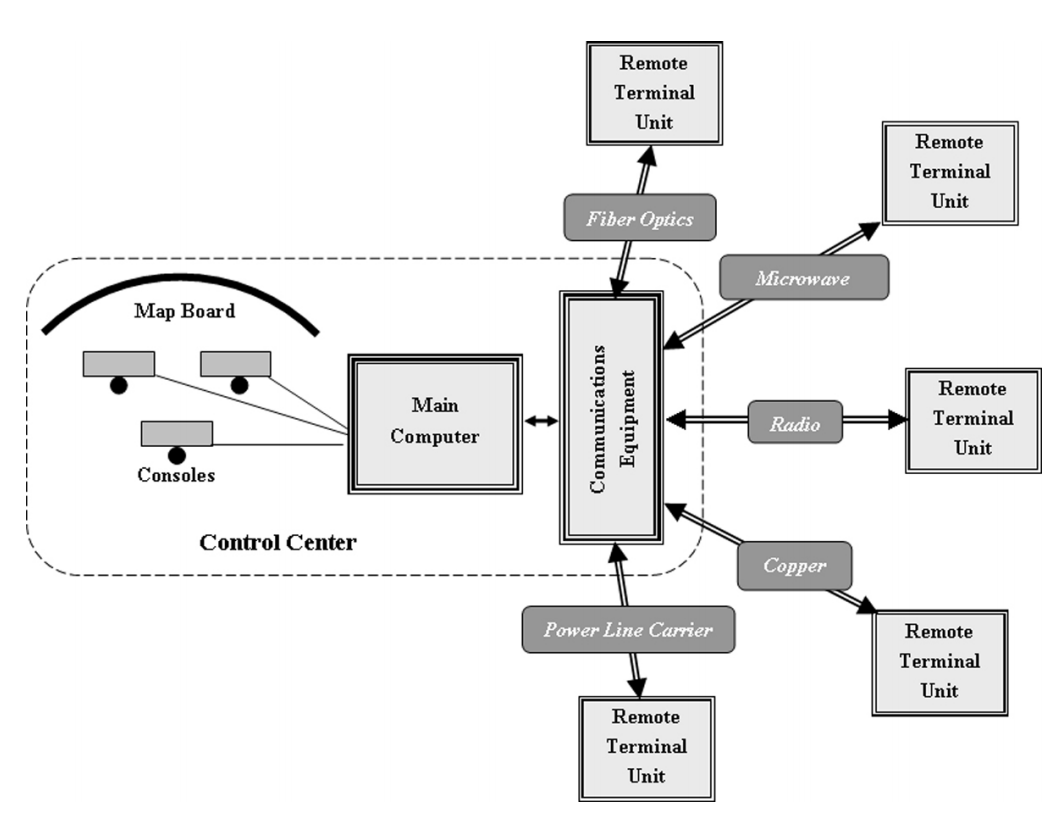
\includegraphics[width=\linewidth]{figures/Blume-SCADA-system.png}
\caption[SCADA system]{SCADA system , as presented in \cite{BlumeStevenW2007Epsb}}
\label{fig:Blume-SCADA-system}
\end{figure}

%[ \fullcite{el2008introduction} ] \\ 


A centrally located control center, optionally being backed up by control centers at one or more locations for redundancy, displays status information from the equipment at the associated substations, received for monitoring purposes. As a response to alarms indicating operational issues, commands enabling remote control of affected infrastructure is issued in order to address the issue, in order to resolve the issue and receive updated status information clearing the alarm. 




%\section{Description}
%- WAMS description

\section{The Smart Grid Control System}


\subsection{Introduction}

Analogous with the modernisation of the classic \acrlong{pg} into the \acrlong{sg}, the \acrshort{scada} subsystem of the \acrshort{pg} is the predecessor of the control system of the modern \acrlong{sg}.
Therefore, a description of the \acrshort{scada} system, evolving from the centralised subsystem controlling the Classic \acrshort{pg}, to the modernised version of the \acrshort{scada} subsystem, initiates the description of the \acrlong{sg} Control System. 




The characteristics of the three generations of SCADA systems% described by \Citeauthor{alcaraz2012security} in \cite{alcaraz2012security},
may be summarised below:
 

 \begin{enumerate}
     \item A Monolithic SCADA system utilises a centralised offline control center  infrastructure, in order to monitor and control the physical system by proprietary control mechanisms.
     \item A Distributed SCADA system utilises a networked, but centralised control  center in order to monitor and control the physical system by proprietary control mechanisms. 
     \item A Networked SCADA system utilises a networked, and online control  center in order to monitor and control the physical system by standardised control mechanisms.
 \end{enumerate}







\subsection{The Modernised SCADA system}
 
 The \acrshort{scada} system is%, as described in \cite{alcaraz2012security},
 a system utilised to supervise and control \acrfull{ci} systems, including \acrshort{pg} infrastructures. Initially designed in order to control physical infrastructure systems like the classic \acrlong{pg}, the Monolithic SCADA system emerged into the Distributed SCADA system. The transition from a Monolithic SCADA system to a Distributed SCADA system transforms, as indicated by %figure \ref{fig:SCADA-CentralisedAndDistributed}
 , the central management center from a centrally controlled mainframe environment, to a networked server environment controlled by operators connected through a \acrfull{lan}
  
  
 The \acrshort{sg} control center emerged from the Distributed SCADA system, into the Networked SCADA system used in order to control modern \acrlong{cps}s, like the \acrshort{sg}.\\ 
 


 





 




However, as explained by \Citeauthor{zamani2020introduction} in \Cite{zamani2020introduction}, the \acrshort{scada} system has a number of shortcomings, making it unsuitable for a \acrshort{sg} enegy distribution monitoring system:

\begin{itemize}
    \item The data polling rate is once every 2-10s, which is not sufficient in order to get real-time measurements.
    \item No time-stamps are attached to samples, making it hard to monitor rate of change over time
    \item State Estimation is not performed with sufficient frequency, if at all.
    \item The ability to observe dynamics is not supported by the system.
\end{itemize}





In order to address these shortcomings, the \acrfull{wams} system\footnote{WAMS is also known as the Wide Area \textbf{Monitoring} System}, described next, was invented.






\subsection{Description of the Smart Grid  Control system}
The \acrlong{sg} system constitutes a complex system of subsystems, which proper operation is a prerequisite for the successful transmission of electric energy from producers to consumers, according to the current demand for energy, as controlled by the Demand Management system, dynamically adjusting the energy supply accordingly. In order to successfully reply to the dynamically changing demands for energy, a close monitoring of the production and transmission of energy through the Wide Area network is required. \\ 

The \acrshort{sg} consists of a vast number of both conventional and modern, more dynamic, production facilities, which requires thorough monitoring in order to ensure the optimal distribution of electrical energy. The requirement of a consistently stable and reliable supply of energy is constant, while the amount of energy demanded is dynamically changing according to the demand for power at any time. \\ 

Therefore, the proper \acrshort{sg} operation might be considered virtually impossible without a  close monitoring of current power flow, as well as the ability to instantly adjust the supply of power according to present needs,  without the risk of causing power surges or blackouts. For this purpose, the Wide Area Monitoring System analyses the levels of electrical power as monitored by sensors, synchronised according to a common GPS-controlled time source. \\ 

The correctness of this time source is critical to the reliability, and therefore, the proper operation of the monitoring system, constituting the primary decision criteria for actions controlling the supply of power.






\
% In \cite{el2018cyber}, \citeauthor{el2018cyber} ...
 


%\subsection{Threats to security}
%In order to ensure the continuous operation of the \acrlong{sg}, identifying security vulnerabilities, and countering threats identified is of vital importance.  




\section{Advantages}
%  - advantages
\section{Security Issues}
%  - security issues
%\subsection{WAMS Security} 

The \acrfull{sg} \acrfull{wams} is a \acrshort{sg} subsystem enabling \acrshort{sg} system operators to monitor the state of \acrshort{sg} energy flow, and general system state. 
A vital requirement for the view of the current state of the \acrshort{sg} energy distribution to be correct is, as described in previous chapters, the ability of the \acrshort{wams} Super \acrshort{pdc}  to utilise synchrophasors collected from the \acrshort{pdc}s to produce a view of the system state. In order for the view to be correct, however, the correctness of the timestamps i critical.  Therefore, in order to produce correct time stamps, the reliability of the Time Synchronisation source is of Critical importance.


\section{State Estimation}

%  - State Estimation: Intro, to explain means to improve grid security.

%\section{WAMS state estimation}
In order to monitor 

\section{Wide Area Measurement System}
\begin{figure}[ht]
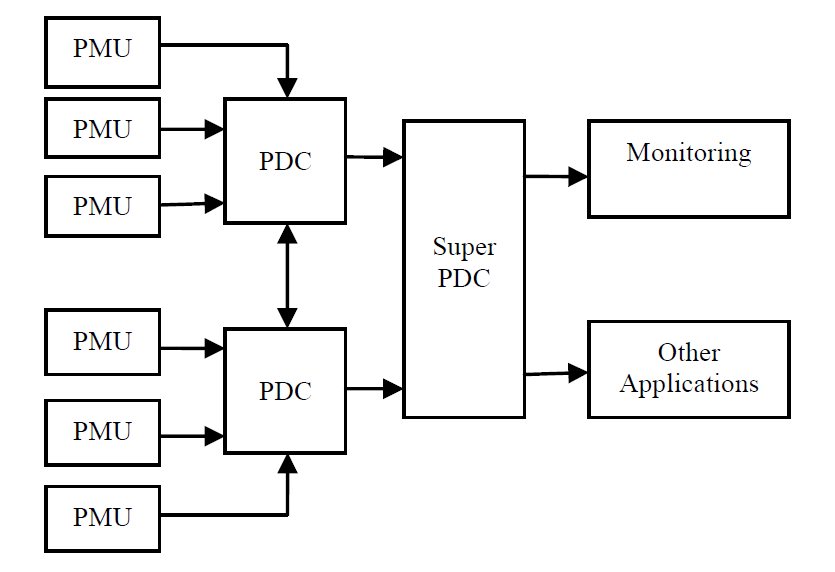
\includegraphics[width=\linewidth]{figures/Kumar-WAMS-architecture.png}
\caption[WAMS architecture]{WAMS architecture, as presented in \cite{kumar2015monitoring}}
\label{fig:Kumar-WAMS-architecture}
\end{figure}










\textit{DESCRIPTION:}
\textbf{\cite{kumar2015monitoring} \fullcite{kumar2015monitoring} }


    

In order to ensure the continuous monitoring of the modern \acrlong{sg} energy distribution system, the \acrfull{wams} is utilised. An overview of the \acrshort{wams} architecture, as presented in   \cite{kumar2015monitoring}, is shown as \figureautorefname  { } \ref{fig:Kumar-WAMS-architecture}:

The \acrshort{wams} is, as described in  \cite{kumar2015monitoring}, a  system, consisting of:

(1) \acrshort{pmu}s, (2) \acrshort{pdc}s, (3) The super \acrshort{pdc}, and (4) Communication networks.

The various components might be described as follows, from (4) to (1):
\begin{itemize}
    \item The \textbf{Communication Networks}, providing data transport between \acrshort{wams} components, as required.
    \item The \textbf{Super \acrshort{pdc}} controls several \acrshort{pdc}s constituting a distributed \acrshort{wams}.
\item The \textbf{\acrfull{pdc}} is responsible for collecting and interpreting \acrshort{pmu} measurements, before synchronising the measurements according to timestamps, in order to get more complete status information based on a combination of measurements.
    \item The \textbf{\acrfull{pmu}} is an intelligent measuring device, responsible for registering sensor measurements,  performing calculations like, for instance, phase angles, as well as voltage and current magnitudes. The data registered and processed by the \acrshort{pmu}, is transferred to the nearest \acrshort{pdc}.
    \end{itemize}

\begin{figure}%[ht]
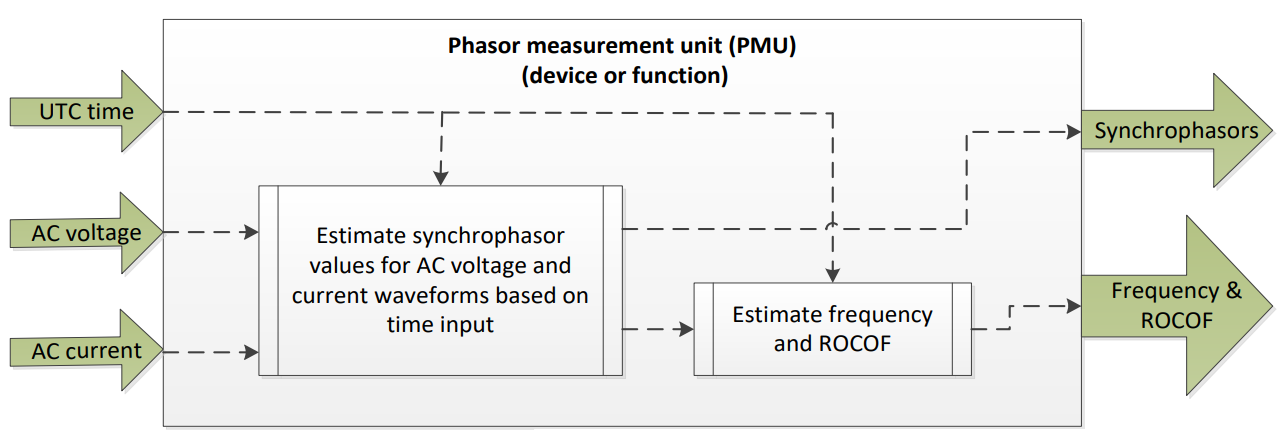
\includegraphics[width=\linewidth]{figures/PMU-in-out.png}
\caption[PMU inputs and outputs]{PMU inputs and outputs, as presented in \Cite[p.12]{iec2018measuring}
}
\label{fig:PMU-in-out}
\end{figure}

\begin{figure}%[ht]
    \centering
    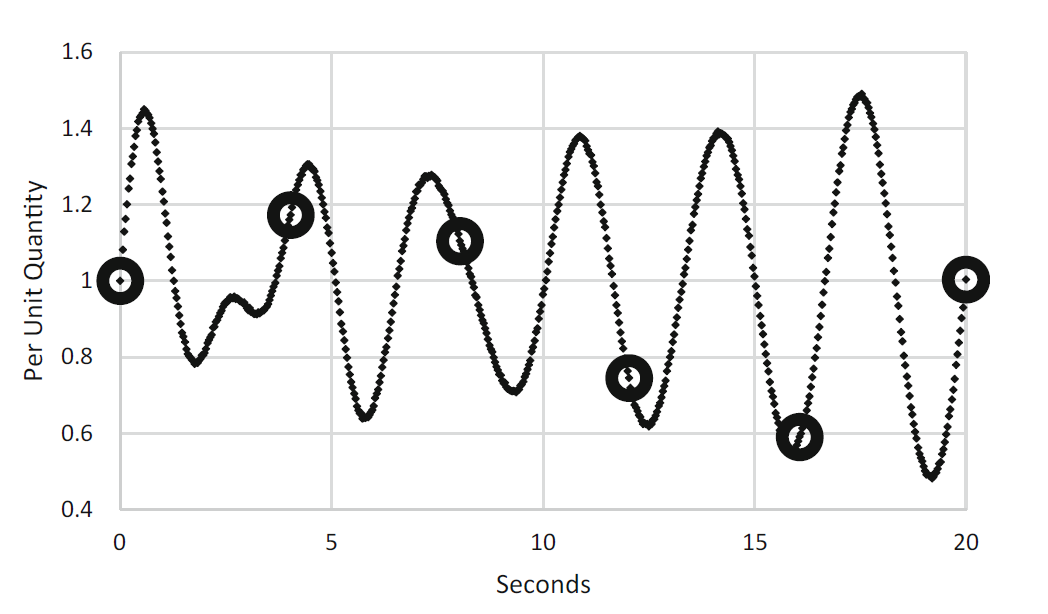
\includegraphics[ width=\textwidth]{figures/syncrophasors-vs-scada.png}
    \caption[Difference between Synchrophasor and SCADA measurements]{As presented in \cite[p. 3]{dagle2019importance}: Notional representation of the difference between synchrophasor and SCADA
measurement. Figure credit: \citeauthor{dagle2019importance}}.
    \label{fig:syncrophasors-vs-scada}
\end{figure}  

\chapter{Smart Grid Power Flow Status Monitoring}

The \acrshort{sg} consists of a vast number of both conventional and modern, more dynamic, production facilities, which requires thorough monitoring in order to ensure the optimal distribution of electrical energy. The requirement of a consistently stable and reliable supply of energy is constant, while the amount of energy demanded is dynamically changing according to the demand for power at any time. \\ 

Therefore, the proper \acrlong{sg} operation might be considered virtually impossible without a  close monitoring of current power flow, as well as the ability to instantly adjust the supply of power according to present needs,  without the risk of causing power surges or blackouts. For this purpose, the Wide Area Monitoring System analyses the levels of electrical power as monitored by sensors, continuously sampled and forwarded to the \acrshort{wams}, through  a networked infrastructure continuously time-synchronised within a fraction of a second tolerance, for the less demanding subsystems.


The correctness of this time source is critical to the reliability, and therefore, the proper operation of the monitoring system, constituting the primary decision criteria for actions controlling the supply of power.




\section{Time Synchronisation}

In order to be able to synchronise events in time, it is mandatory to adjust the clock of each participating actor, analogous to the classic pre-operational physical watch-synchronisation meetings in the physical domain. \\ 

The \acrshort{sg} time synchronisation requirements are, to say the least, a bit more demanding than a simultaneous(-ish) press on buttons to start timing from a common time reference.

Several articles, of which \cite{appasani2018review} may serve as an example, stresses the importance of utilising a precise and reliable times source.

%
  %Given the distributed nature of the \acrshort{pmu} devices providing samples from locations distributed over a Wide Area Network, the \acrfull{gps} is the  time source selected. 


\subsection[Smart Grid Time Sync Precision Requirements]{Smart Grid Time Synchronisation Precision Requirements}

In order to ensure the time precision required for the \acrshort{sg}, the correct selection of time synchronisation mechanisms is vital. 










\subsection{The Importance of Time Synchronisation}

In \cite{dagle2019importance}, \citeauthor{dagle2019importance} states the following aspects as the benefits for Smart Grid operation, of ensuring correct time synchronisation:


\begin{itemize}
    \item  Situational Awareness and Wide-Area Monitoring
    \item  Real-Time Operations
    \item  Power System Planning 
    \item  Forensic Event Analysis
    
\end{itemize}

\subsection{Possible effects of Time Synchronisation errors}
Timing errors will, according to ,,, render the data introduced to the \acrshort{wams} system inadequate to enable \acrshort{sg} operatiors to get overview of the Energy supply state of the \acrshort{sg}.

In \Cite{martin2019impact}, \citeauthor{martin2019impact} lists a number of side-effects which could result form the absence of high-quality data material from the \acrshort{wams}.


\begin{enumerate}




    \item Data loss,
    \item Data corruption,
    \item Inaccurate representation of engineering quantities,
    \item Lack of precision,
    \item Incorrect measurement identification,
    \item Excessive or inconsistent latency.

\end{enumerate}






\section{WAMS Time Synchronisation}



The \acrlong{wams} is critically dependant on precise Time Synchronisation, as a Time Synchronisation error of a few $\mu$-seconds may result in \acrshort{sg} monitoring instability. The time stamps produced by Synchrophasors, pinpointing the exact time of any system event, is vital in order to ensure precise and reliable system state information.
In the event of a system alert being triggered by erroneous system state Information, corrective actions by operators might have undesired effects. In order to synchronise the samples received from the \acrshort{pmu}, the \acrshort{pdc}, as well as the \acrshort{pmu} devices producing the samples, is vitally dependant on precise timing adjustments, in order to establish a precise and correct overview of system state. Incorrect synchronisation of measurements caused by erroneous timing information, will produice an equally wrong system state overview, as presented in the \acrshort{sg} \acrshort{wams}. \\ 


\section{Protocols}
A large number of protocols are defined, in order to standardise the operation of the \acrlong{sg}.

A small selection of these, relevant for the scope of the thesis, are described underneath.

\cite{2021arXiv210311657E} \hl{describes communication protocols} in the  \acrshort{sg}.













\section{Time Synchronisation Protocols}


Time Synchronisation protocols are used in order to synchronise the time of interconnected devices in need of synchronised time for various purposes. In the case of synchrophasor devices, the devices needs to be time synchronised in order for \acrshort{sg} \acrshort{wams} operators to get a correct overview of the system state.

\subsection{Time Synchronisation Protocols Presicion Requirements}
Time synchronisation protocols are controlling the synchronisation of time between various devices of the grid, like the PMUs, collecting phasor measurements from a definde number of measuring devices. Synchronised time is crucial in order to ensure each PMU is able to put the correct time stamp on each phasor measurement, before transmitting the resulting synchrophasor for each time stamp, to the destined PDC device. In the event one of the synchrophasors have an erroneous time stamp, an error affecting the integrity of the synchrophasor data is introduced. As described in \cite{moussa2016security}, \acrlong{ptp} synchronisation network
, as well as \acrlong{gnss} based synchronisation networks, are both capable of producing the precision required by the synchrophasor protocols, as opposed to the more common \acrfull{ntp} commonly used in ordinary computer networks. As my thesis covers \acrshort{ptp} time synchronisation only, my description of time synchronisation protocols is limited to the \acrfull{ptp}.



The \acrshort{ptp} is included in the IEC standard

%\subsection{Synchrophasor data alignment attack}
Eq \ref{DMS} about DMS, and  eq \ref{DSM} about DSM.









%Unlike the \acrlong{cpg}, the \acrlong{sg} enables bidirectional flow of power, by customers operating micro grids enabling customers to sell excessive power back to the network.








%\section{Historical}
%SCADA monitoring flaws -> PMU




%\section{PMUs}
%PMU
%-  Descripton of PMU
%- phasor
%- synchronised phasors
%- Communication with PDC

%\section{PDCs}
%PDC
%- Collecting synchronised phasors from PMU
%- Grouping synchronised phasors with same timestamp into Synchrophasor record
%- At deadline, transmitting Synchronaised phasors, received before deadline.
%- Improved security. 
%\section{Synchrophasors}
%Synchrophasors
%- overview
%- sync precision requirements:
 
%\section{Protocols used for monitoring}
%Protocols
%- Figure from PowerPoint
%- Concentrating on upper left side of figure.


%- capabilities of x.2011 x=synchrophasor protocol

%PTP
%Rationale for concentrating on PTP
%Descriptino of the protocol
%Time synchronisation via PTP
%PTP delay attack (types)



\subsubsection{Precision Time Protocol services}
The \acrfull{ptp} is a network-based time protocol, enabling the time difference between devices to be synchronised within a fraction (in the order of a few $\mu$s) of a second, satisfying the requirements of the \acrshort{sg}. 

\begin{figure}[ht]
    \centering
    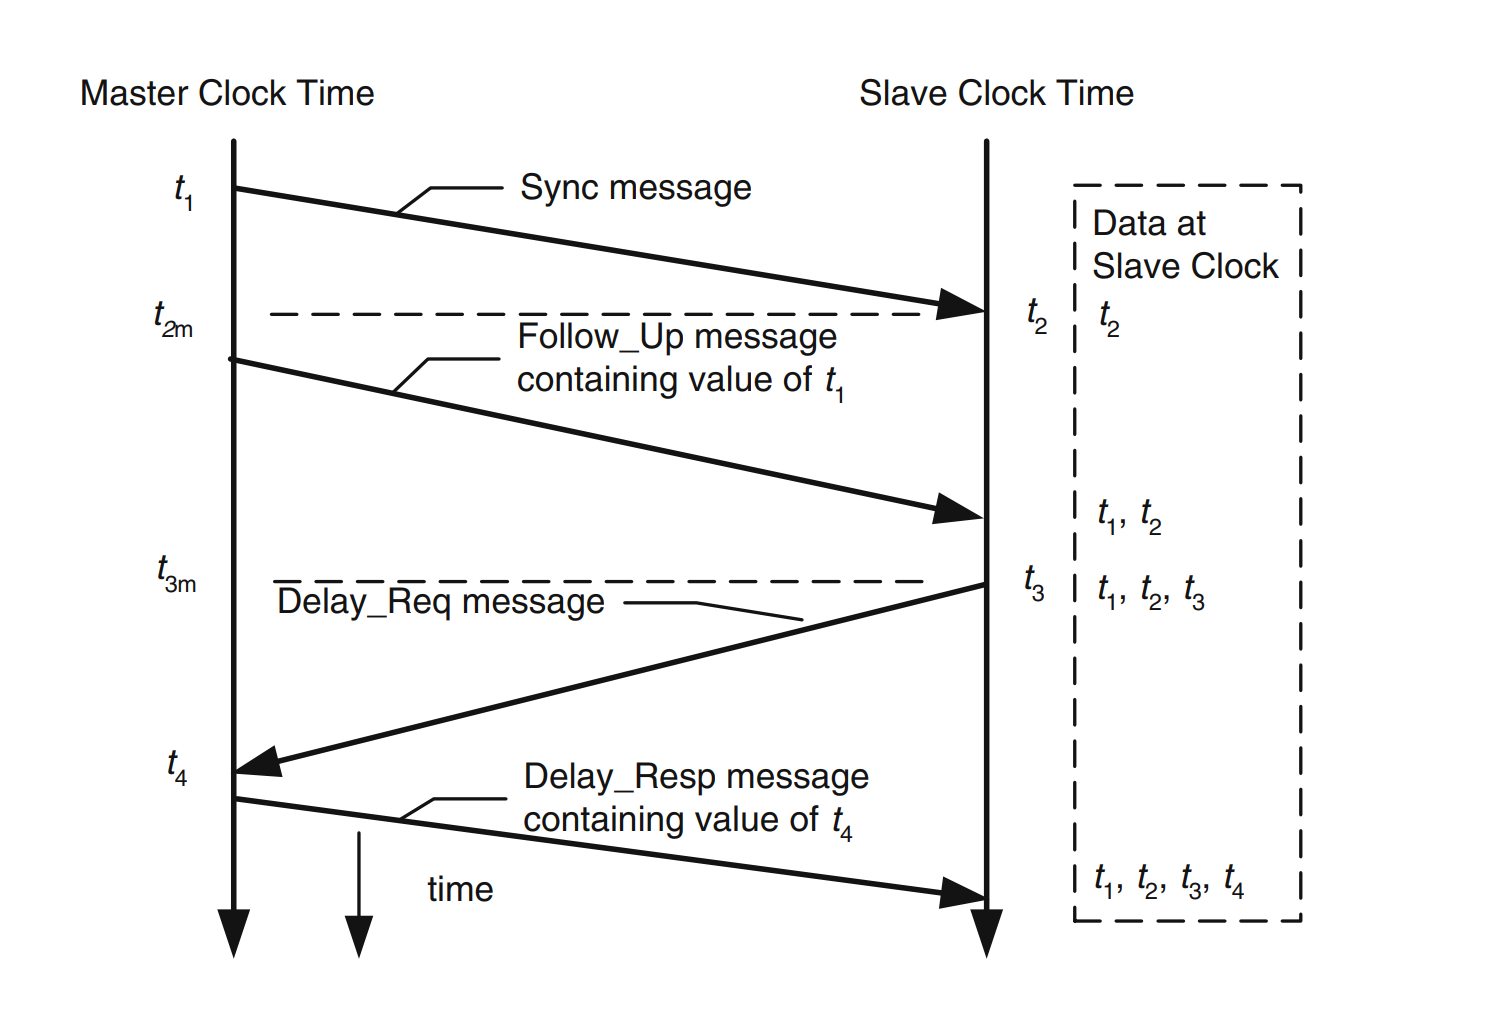
\includegraphics[ width=\textwidth]{figures/PTP-timing-Diagram.png}
    \caption[Timing diagram for synchronization messages]{As presented in \cite[p. 51]{Eidson2006}: Timing diagram for synchronization messages.} 
    \label{fig:PTP-timing-Diagram}
\end{figure}  

\subsubsection{Description of PTP time synchronisation}



A device, being synchronised  by the \acrshort{ptp} protocol, reads its system time from a clock which is continuously synchronised by a network of one or more slave clocks, being periodically synchronised via various types of hybrid\footnote{Hybrid clocks are a master clock for some clocks, while being a slave clock for others.} clocks, ultimately synchronised with a grand master clock.


The time of the slave clock, is being adjusted according to the following process:


Following the message exchange visualised by \figureautorefname { } \ref{fig:PTP-timing-Diagram}, the Slave clock  uses the time offset $\theta$ from the Master clock time, calculated by Equation \ref{eq:offset}, in order to synchronise with the Master clock. 


\begin{equation}
t_1 = t_0 + \theta + d_1 \label{eq:t1}
\end{equation}


\begin{equation}
t_3 = t_2 - \theta + d_2
\end{equation}

\begin{equation}
d_1 = d_2 = d
\end{equation}

\textbf{Bla bla }Equation \ref{eq:t1}

\begin{equation}
%offset
\theta = \frac{(t_2 - t_1) + (t_4 - t_3)}{2} \label{eq:offset}
%\div 2    
\end{equation}
In order to be able to achieve the time difference required, the \acrshort{ptp}, as described by  \citeauthor{Eidson2006}, in \cite{Eidson2006}, is dependant on:

\begin{itemize}
    \item Timestamped network events, messages, which is  used for synchronisation.
    \item A method of timestamp transmission as required for synchronisation.
    \item Overcoming any timing impairments introduced by system components.
\end{itemize}





\subsection{Synchrophasor}
%\cite{ali2016wide}


%\Cite{rana2015exploring}



\begin{figure}%[ht]
    \centering
    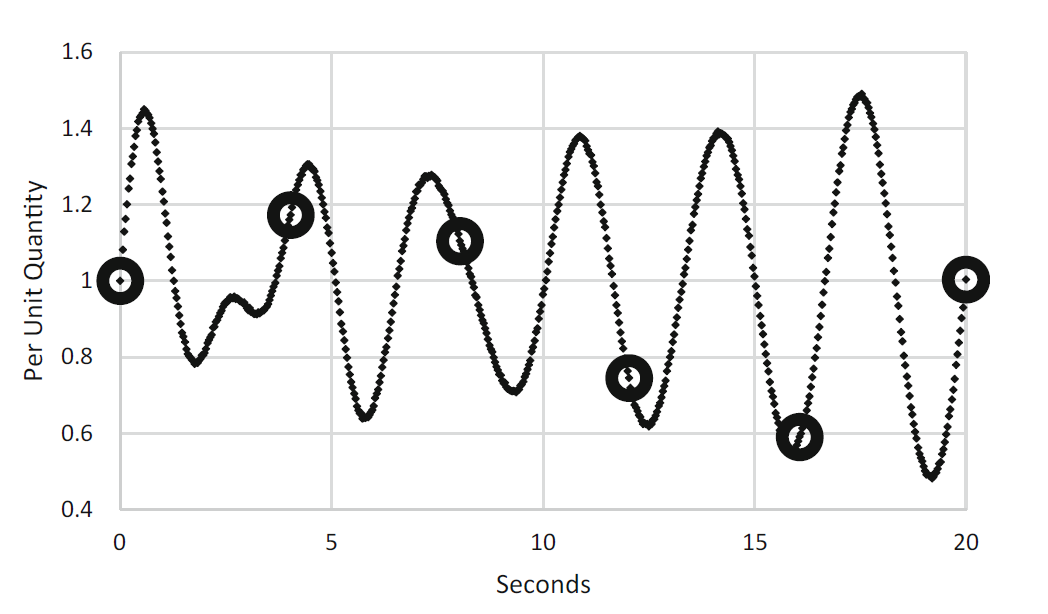
\includegraphics[ width=\textwidth]{figures/syncrophasors-vs-scada.png}
    \caption[Difference between Synchrophasor and SCADA measurements]{As presented in \cite[p. 3]{dagle2019importance}: Notional representation of the difference between synchrophasor and SCADA
measurement. Figure credit: \citeauthor{dagle2019importance}}.
    \label{fig:syncrophasors-vs-scada}
\end{figure}  




The \acrshort{pmu} is receiving values from sensors, on which it is able to calculate voltage level and phase angle of the energy flow. It is utilising a time-source to pinpoint measurements in time, producing synchrophasors, to be transmitted to the nearest \acrshort{pdc}. 

As described by \citeauthor{dagle2019importance} in \cite{dagle2019importance}, the data received from traditional \acrshort{scada} systems are time-stamped after arriving at the control station. The synchrophasors of the \acrshort{wams} on the other hand are, as described by \Citeauthor{ali2016wide} in \cite{ali2016wide}, being time-stamped in real-time before being transferred to the control system. The sampling rate of the \acrshort{pmu}, results in synchrophasor data enabling operators of the \acrshort{wams} to get real-time visualisation of critical elements, like the state of energy flow  of the \acrlong{sg}. The increased granularity of the measurement system allows for the detection of anomalies undetectable by traditional \acrshort{scada} systems, as illustrated by \figureautorefname { }\ref{fig:syncrophasors-vs-scada}. 

The increased sampling rate, of the synchrophasors of the \acrshort{wams} systems enables a more fine-grained view of energy distribution system state changes. However, in order for the \acrshort{wams} system to get the correct system state information, correct time stamps is critical. 
Therefore, the time-synchronisation mechanisms of the \acrshort{pmu} system is of critical importance. \\ 

\begin{figure}
    \centering
    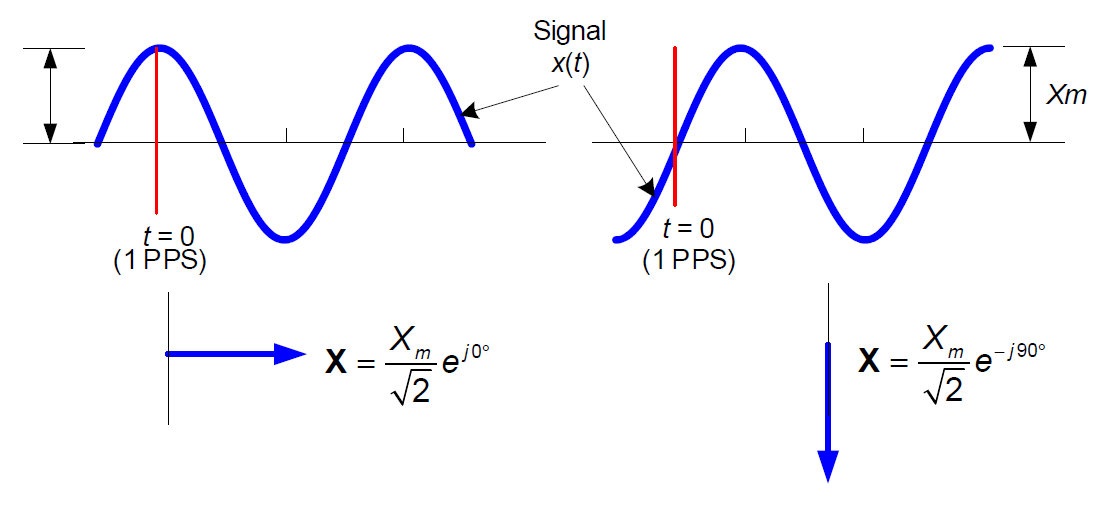
\includegraphics[ width=\textwidth]{figures/Synchrophasor-Definition.png}
    \caption[Convention for synchrophasor representation]{As presented in \Cite{schofield2018design}: Convention for synchrophasor representation.}.
    \label{fig:Synchrophasor-Definition}
\end{figure}  




\subsection{Synchrophasor Protocols}

\hl{The introduction of Synchrophasors in the} \acrlong{pg}, 

\subsubsection{Introduction}



As described in \cite{martin2011synchrophasor} and \cite{ali2016performance}, the \acrfull{pmu}, along with the \acrfull{pdc}, were introduced in the 1980s. The communication and data exchange from the PMU to the PDC was standardised by the introduction of the IEEE 1344 standard in 1995, which was established as the standard communication protocol for synchrophasor data exchange. According to \cite{appasani2018review}, the IEEE 1344 was revised in 2001 , before the introduction of the IEEE C37.118 in 2005. The  IEEE C37.118 protocol was derived from the IEEE 1344 standard, and has undergone a number of revisions, over the years.


In \cite{martin2013synchrophasor}, \citeauthor{martin2013synchrophasor}describes the history of the 
IEEE C37.118-series of satndards. The characterisitcs of the various generations, might be summarised as:
\begin{itemize}
    \item The IEEE C37.118-2005,
    \item The IEEE C37.118-2011
    \item The IEEE C37.118-2018
\end{itemize}






\chapter{Smart Grid Cyber attacks}
%Overview of cyber attacks
%\section{Threat Actors}
%Threat actors
%- Threat actor Categories
%  - MitM
%  - MotS
%- Threat actor Capabilities

%\section{Types of Cyber Attacks}
%Cyber Attacks
%- Cyber Attack Categories
%  - (D)DoS
%  - FDI
%  - Time Delay Attack
%  - Malware





%\chapter{Cyber Attacks on the Smart Grid}









The \acrfull{sg} is a complex system delivering electrical power to a society more dependant on electricity then ever, given the transition from traditional sources of energy to electrical energy on areas like agriculture, industrial production, heating, and more recently, transportation.
The transition of the electrical grid from the classic \acrlong{pg} to the \acrlong{sg} exposed, as previously described, the \acrlong{ci} of the power grid to attacks from remote locations via the Internet. 


\section{Attack via time protocols}

Computer systems reachable\footnote{Systems could ultimately be targeted utilising USB sticks, if not accessible from the Internet.} from the outside world,  are potential targets of Cyber attacks. The eventual recoveries of the initial Cyber Attacks was followed up by defence actions, resulting in more advanced attack techniques, has evolved to a continuous battle of control between attackers and defenders. \\


\subsubsection{Threat Actor  Types}
There are numerous Threat Actors of various skill levels, from so-called "Script Kiddies" to professionals, aiming to get unauthorised access to systems, for fun, fame, or for more serious reasons, like terrorism or financial gain. 

\begin{itemize}
    \item The \textbf{Internal attacker} has privileged access to, at least parts of, the internal infrastructure of the target, enabling the ability to take malicious actions not available to non-internal attackers.
    \item The \textbf{External attacker} is limited to attacking the targeted infrastructure from the outside, typically through network connections.
    \item The \textbf{Traffic Injector attacker} adds network packages to the benign traffic of the networks of the target, in order to produce the desired effects on the state and operation of the targeted infrastructure. 
    \item The \textbf{\acrshort{mitm} attacker} interrupts the communication between the two parties A and B, impersonating as B to A and vice-versa.
    \item The  \textbf{\acrshort{mots} attacker} are able to eavesdrop on communications, without any privileged access to enable the direct modification of any data transmitted.
\end{itemize}



The various types of attackers possesses various malicious action capabilities, which they may use in order to attack their intended target in numerous ways.


%\subsection{Time  Protocol Threats}










\subsection{Examples of Cyber attacks}
As described in \cite{sundararajan2019survey}, a number of security incidents targets the \acrshort{sg} specifically, like the 2015 BlackEnergy3 attack on the Ukranian  Power Grid, the StuxNet worm of 2010, as well as the watering-hole remote access trojan attack of 2014. 
Any online \acrshort{sg} infrastructure containing vulnerabilities, is equally inflicted by attacks not specifically targeting \acrfull{sg} like the WannaCry ransomware cryptoworm of 2017, targeting the EternalBlue vulnerability of unpatched windows computers.







%\subsubsection{Time Synchronisation attacks}
\section{Cyber Attacks targeting Smart Grid}

The two-way communication lines of the\acrlong{sg} systems opens the possibilities of communication between the networks of energy distributors and the networks of consumers, serving purposes as automatic measurement of energy consumption, as well as dynamic adaption of energy production according to variations in demand for energy over the hours of the day.
The transition from networks managed by closed communication channels to networks communicating over IP-based networks, exposes\acrlong{sg} networks to Cyber attack vulnerabilities.
Malicious threat actors having privileged access to the infrastructure, is able to perform various kinds of internal attacks.\\

Traditionally, anyone aiming to attack the \acrlong{pg} infrastructure, was obliged to get physical access to the premises, from which the infrastructure in question was controlled. Following the transition to the online \acrshort{sg}, the network connecting the grid to the outside might be utilised in order to execute any Cyber attack requiring internal privileged access from the outside.


\subsection{External Attacks}
External attacks is characterised by malicious actors attacking the infrastructure from the outside, without having the privileged access required in order to target internal system vulnerabilities.


\subsection{Internal Attacks}
The distinction between external and internal attacks, is the level of access required in order to perform the attack in question.

\subsubsection{Man on The Side (MoTS) Attack}
The \acrfull{mots} attack is a type of attack requiring minimal privileges and system access in order to be successfully executed.




\begin{figure}
    \centering {
    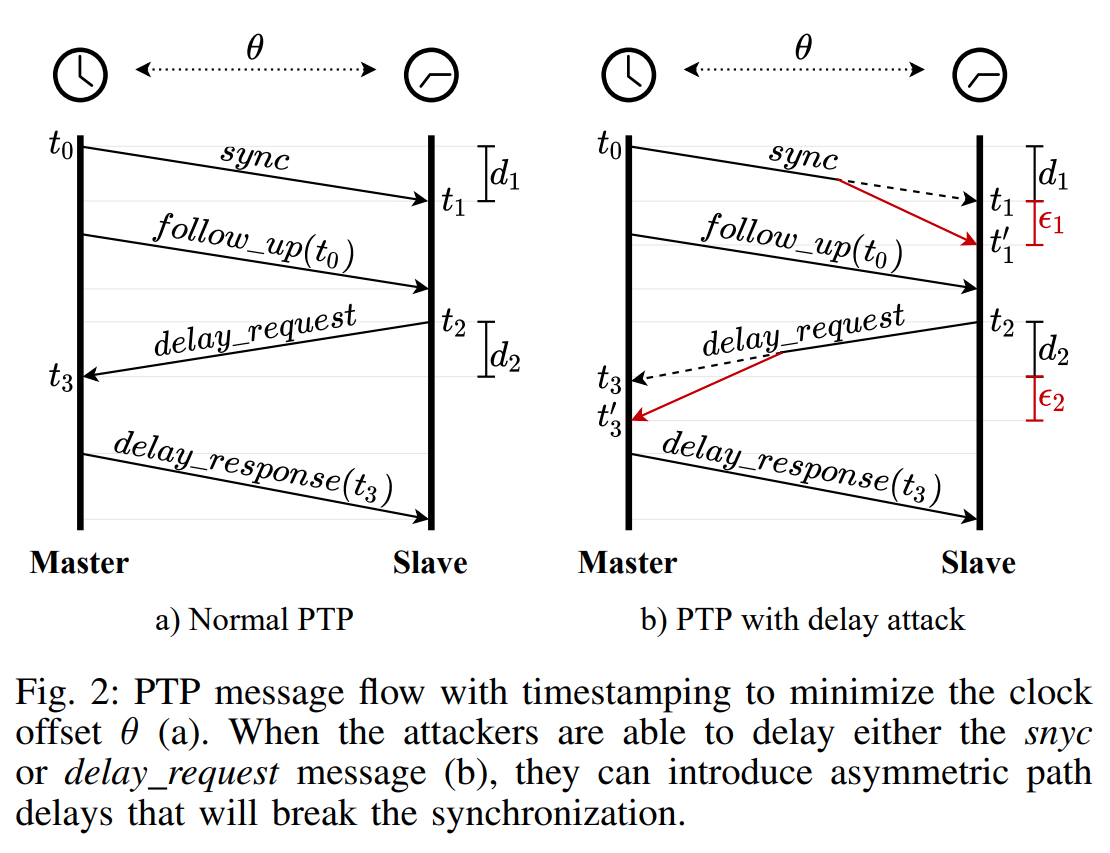
\includegraphics[ width=0.9\textwidth]{figures/PTP-delay attack.png}
    \caption[PTP Sync: Normal sync vs. sync under PTP Delay attack]{As presented in \cite{finkenzeller2022feasible}, figure 2. Comparison of PTP delay attack synchronisation with normal PTP synchronisation.}
    \label{fig:PTP-DelayAttack}
  }
\end{figure}  



\section{PTP delay Attacks} \label{sec:PTP-delay}
Several attacks which targets the \acrlong{ptp}  utilises vulnerabilities in the PTP, as explained by \cite{finkenzeller2022feasible}:


Based on the equations related to the regular \acrshort{ptp} synchronisation, in \cite{finkenzeller2022feasible} stated as:



\begin{equation} \label{eq:5-t1}
t_1 = t_0 + \theta + d_1 
\end{equation}

\begin{equation} \label{eq:5-t3}
t_3 = t_2 - \theta + d_2 
\end{equation}

\begin{equation}   \label{eq:5-d1}
d_1 = d_2 = d  
\end{equation}

%\textbf{Bla bla }Equation \ref{eq:5-t1}

\begin{equation}  \label{eq:5-offset}
\theta = \frac{(t_1 - t_0) - (t_3 - t_2)}{2}
\end{equation}


\begin{equation}  \label{eq:5-d}
d  = \frac{(t_1 - t_0) + (t_3 - t_2)}{2}
\end{equation}


The PTP delay attack uses the following equations:

\begin{equation}
    t'_1 = t_0 + \theta + d_1 + \epsilon_1
\end{equation}


\begin{equation}
    t'_3 = t_2 - \theta + d_2 + \epsilon_2
\end{equation}


Using the equation \ref{eq:5-d}, we arrive at  the following equations:



\begin{equation}  \label{eq:5-dtheta}
\theta' = \frac{(t_1 - t_0) - (t_3 - t_2)}{2} - \frac{\epsilon_1 - \epsilon_2}{2}
\end{equation}

\begin{equation}  \label{eq:5-d-delay}
d' = \frac{(t_1 - t_0) - (t_3 - t_2)}{2} - \frac{\epsilon_1 + \epsilon_2}{2}
\end{equation}

and accordingly:
\begin{equation}
    \theta' = \theta - \frac{\epsilon_1 - \epsilon_2}{2} 
\end{equation}

and \\

\begin{equation}
    d' = d - \frac{\epsilon_1 + \epsilon_2}{2} 
\end{equation}


For the attack, \citeauthor{finkenzeller2022feasible} further describes, the attacker has the option to set the desired (erroneous) clock offset value at will, as well as being able to control the offset direction. choosing vvalues of $\epsilon_1$ and  $\epsilon_1$ as $\epsilon_1 < \epsilon_2$  for setting the slave behind, whereas the reverse is true for the case of  $\epsilon_1 > \epsilon_2$. \\ 

Thus the \acrshort{ptp} delay is a realistic attack. Some of the various flavors of the attack should be obtainable for an attacker having limited access to the Target of the attack, like a \acrfull{mots} attacker.
\chapter{Method} 

%The method chapter should describe in detail which activities you undertake to answer the research questions presented in the introduction, and why they were chosen. This includes detailed descriptions of experiments, surveys, computations, data analysis, statistical tests etc.

\section{Introduction}


As a background for the thesis, a scenario where a threat aactor
 In a preliminary phase of the attack, a phase of attack simulation will provide useful information, aiming to learn more about detection probability, as well as some empirical background for the evaluation of possible consequences.
The potential outcome of the simulation may be used in order to prepare for attacking the actual infrastructure with attacks with a low attack detection probability and, to the best possible knowledge, with foreseeable consequences of the attack.

As described previously, the aim of the thesis is to investigate any observable effects of specific time delay attack simulations. Such simulations could be executed in a preparation phase, preparing for the execution of an actual time delay attack.

 \textbf{Some papers} describes a number of varieties of the PTP delay attack, while \textbf{other papers} describes the attack to have severe consequences to the \acrshort{sg} infrastructure. The primary goal of the actual attack is to stay undetected, while exposing the infrastructure under attack to an attack having the most severe consequences possible, while still avoiding detection.  
 


As part of the introductory studies of the topic selected, a couple of searches on the NTNU literature search facilities returned a number of books, like \cite{BlumeStevenW2007Epsb} and \cite{kabalci2019smart}, covering introductory chapters on Power Grid and Smart Grid. The introductory chapters heavily relies on descriptions from relevant book chapters. 


%For the \acrfull{wams} Security parts, a small number of surveys, as well as a collection of papers are investigated, covering  synchrophasor protocol attack vulnerabilities, highlithing some known side effects of successful synchrophasor protocol attacks. The introductory brief coverage of \acrshort{sg} security, is followed by a coverage of common synchrophasor protocols, focusing on attack vulnerabilities of the protocols covered. \\ 






%Several test cases utilising PMUs and PDCs



%In order to investigate, systems like mininet. \\ 


\section{Research Design}
%This section will inform the reader of the NATURE of your study. In other words, broadly speaking: are you aiming to describe a phenomena (descriptive design), are you aiming to explore a topic (exploratory design), are you looking to identify causal relationships between factors (causal design)?

%The aim of the thesis, is to present an overview of concepts, as well as to to provide examples from the literature related to the Smart Grid WAMS being vulnerable to attacks on the Synchrophasor protocols. 
In order to be able to observe the effects of exposing a \acrshort{pmu} to a time delay attack, the real attack is dependant on getting access to expensive equipment, like a \acrshort{pmu} as well as the interconnected infrastructure.
As previously discussed, a time delay attack on Synchrophasors imposes a high risk of causing damage to the infrastructure targeted.
Given the high potential for damage, a good option for visualising any potential effects a time delay might have on the values produced by a \acrshort{pmu} under attack, would be to simulate the attacks.
There exists a number of projects which utilises MATLAB and SIMULINK in order to model power grid components in general and, specifically, \acrshort{pmu}s.



In order to 

Based on the findings of the initial literature study concerning vulnerabilities, the literature study continues providing potential scenarios for stealthy MiTM attacks on the synchrophasor transmission system, investigating the success of the attacks maximising side effects while minimising the probability of being detected.

As the final part of the thesis, a theoretical discussion, aiming to provide answers to the research questions, will be conducted.\\ 

\textbf{TO DO:}
\textit{As a experimental part of the thesis, possibilities of testing one or more detection and mitigation techniques might provide a contribution to the final discussion and conclusions based on my own experimental results}


\section{Research Methods}

%Following the description of your research design, you should also devote a section to describing the research methods you applied during your study. Each design will provide you with many possibilities of methods to use.

In order to provide theoretical evidence on which to answer the research questions, a literature study will be conducted.
For any experimental results, experiments will be described, implemented and executed.

\section{Measurements}

%Once you clarified the method you used, it is time to explain exactly WHAT you measured (e.g. service quality, brand image, satisfaction, purchase intention) and HOW you measured

Vulnerability to time-shift attacks are quantified by articles describing theoretical aspects of the mechanisms for the calculation of valid time-stamps, and the inherent tolerance level for calculation errors. Modern Smart Grids require the time deviating from the correct time by a fraction of a millisecond. Specifically, according to \cite[p.  1953]{moussa2016security}, the allowed time deviation for a 50Hz electrical system\footnote{As used in Norway, for instance} must be within $\pm$31.8 microseconds, in order to adhere to the 1$\%$ \acrfull{tve} requirement, as specified by the  IEEE C37.118 standard. \\ 

Experimental investigations reported by articles selected will be provided as relevant examples, in order to support any discussion arguments for the purpose of reaching conclusions.  

\section{Sample}

%In this section you should detail (at least!) the population of your study, your sampling technique (which technique you used to select the people who took part in your study) and how you established your sample size.
The samples for my literature study will be papers relevant for the discussions, in order to provide answers to the research questions.\\ 

Any execution of experiments will provide experimental samples, with the aim of supporting discussions and conclusions.
\section{Validity and Reliability}

%Now, here is a SUPER important section that 99\% get wrong(I completely made up this figure, simply because I want to convey a point!). Validity (that you measured what you intend to measure) and reliability (that the measurements used, such as your scales, are consistent and replicable) are two concepts that simply have to be addressed and have to do with your measurements.
In order to increase the validity and reliability, a number of articles will be included as the foundation for any conclusions. My personal selection of papers deemed relevant for my discussion, will be selected highlighting on articles being included as relevant articles by survey papers, as well as papers gaining a high relevance score on literature search sites.\footnote{... like the NTNU ORIA site (\url{https://innsida.ntnu.no/litteratur}).} Another selection criteria aiming to increase validity and reliability will be a focus on selecting articles receiving a high number of quotations ratings on sites like Google Scholar. %First and foremost, though, a sound and critical validation of the relevance for the questions at hand is still mandatory. \\  



For the experimental parts, my project is utilising a selection of PDC and PMU simulator packages. In order to validate the phasor data generated, the included validation capabilities of the simulator packages are utilised.

\section{Infrastructure used during experiments }
\textbf{TO DO:}
\textit{A selection of a relevant infrastructure for experiments will be made according to  specific needs and availability.  }\\ 

In order to provide practical results on which to base the discussions and conclusions, the following tools will be utilised;

\begin{itemize}
%    \item The iPMU suite, including iPDC, iPMU and PMUSimulator, running on virtual Ubuntu Linux instances
%    \item The pyPMU suite, including tinyPDC, tinyPMU and , running on virtual Ubuntu Linux instances \cite{vsandi2015python}, \cite{vsandi2016pypmu}
    \item A SIMULINK model, downloaded from \textbf{URL} is used as the basis for the simulations.
    \item MATLAB, \textbf{latest version}, with SIMULINK added, is used for running the simulation. 
    \item The SIMULINK DSP and MATLAB Digital Signal Processing toolkits are required in order to run the simulations.
    \item The \textbf{Model inspector} functionality is used in order to compare the delayed ouput to the original one.
    \item A Windows 10 laptop is being used for the simulations
    
 %   \item mininet will be utilised for networking
 %   \item Wireshark will be utilised for synchrophasor packet analysis
 %   \item Python will be utilised in order to visualise the results

\end{itemize}

%\section{Instruments or Equipment}

%Sometimes, especially in causal studies when researchers are developing experiments, it is important to detail the instruments or equipment that were used in the study.



\section{Simulating a Time Delay attack}



\subsection{Scenarios}

For the experimental part of my thesis, a number of attack scenarios will be required. The aim is to investigate various attack vectors which might be used by a sophisticated man-on-the-side threat actor in order to execute an attack while staying undetected. 

\subsection{Background} 

A number of assumptions is stated, in order to narrow the scope of the thesis.

\subsubsection{Attacker policy assumptions}
A sophisticated threat actor would most likely want to avoid detection by anyone protecting the targeted infrastructure.
Therefore, executing an attack which may be detected should be avoided at all costs.
As a consequence, any decisions related to actually executing the attack should be as a result of promising results following a stealthiness assessment process\footnote{Simulations of possible effects could be part of a stealthyness assessment process}. 

\subsubsection{Attack Prerequisites}
A stealthy attack with small impact is preferred over an attack having more severe impacts, at a higher risk of detection.
The ideal attack would be an attack having maximal impact on the target, while the risk of detection being minimal. 


\subsubsection{Attack design challenges}
A part of the challenge would be to design an attack producing a high impact on the target, while staying undetected.

\subsubsection{selected approach}
One possible solution could be to determine the minimal efforts needed in order to execute an attack with a high probability of producing the effects desired, while keeping the attack detection probability low.



\subsection{Definition of scenarios}
In order to provide experimental results in order to answer the Research Questions stated, a number of attack scenarios are defined.

The main method of simulation would be a delayed forwarding of values, where a specified delay $d$ is applied to the PMU input, replacing any sample $s(i)$ with the sample value $s(i-d)$, simulating clock drift, producing effects similar to a \acrlong{tda}.

The simulation could be performed using a number of delay functions, for instancs:
\begin{enumerate}
   
\item  Exposing the targeted PMU to a constant delay, from a specified initiation time.
    The delay is switched on, unaltered from the time of initiation, for the duration of the simulation. 
\item  Exposing the targeted PMU to a constant delay for a limited time, from a specified initiation time, switching it off during the simulation.  
\item  Exposing the targeted PMU to a increasing delay for a limited time, from a specified initiation time, switching it off during the simulation.   
\end{enumerate}
    


\subsection{Attack Implementation}
%The attacks would be implemented as MATLAB functions executing attacks on targets implemented as SIMULINK simulations. The various scenarios would  be required to be sufficiently similar to be implemented as variations of a single attack framework, in order to avoid the need of creating more than a single attack framework.     

%In order to prepare for attacks, a plan might be to implement the techniques described in \cite{gilad2014off}.



%\textbf{\cite{barreto2016undetectable} proves the requirement of exposing more than two PMUs to a delay attack, for the attack to be undetectable.}




A number of physical investigations related to the effects of any intended attacks on the intended targets, would increase the knowledge of a potentially complex target, increasing the probability of staying undetected during the attack. In order to avoid exposing expensive and critical power system infrastructure to physical damage or downtime,\footnote{In a test lab environment, downtime could be acceptable, whereas the risk of physical damage of typically expensive equipment may be too high, at least not in the initial phases of investigations.} such practical investigations would preferably be performed in a simulation environment.

\section{Creating a Simulation environment}

This approach could be taken by a threat actor during a phase of investigations in the preparation of the actual attack, for the purpose of learning more about the possible consequences of performing intended actions on the intended target. One of the most important priorities of the threat actor, is to stay undetected for as long as possible. Simulations are designed in order to investigate the selected attack scenarios. The planned attack is implemented using a combination of Simulink and MATLAB. The execution of each simulation will produce corresponding graphs, illustrating any visible effects the attack may have on the system, by analytically comparing the output produced by the attack, with the alternative output of the unmodified, and correct Synchrophasor signal corresponding to  a situation of no attack being performed.

\subsection{Modelling a PMU}

As the plan of the threat actor is to expose  a number of \acrshort{pmu}s to a time  delay attack, the plan is to build a model of a \acrshort{pmu}, allowing the model to be run while altering any time stamp values required, in order to investigate any observable effects on the output from the \acrshort{pmu}.
 \begin{figure}[ht]
\centering
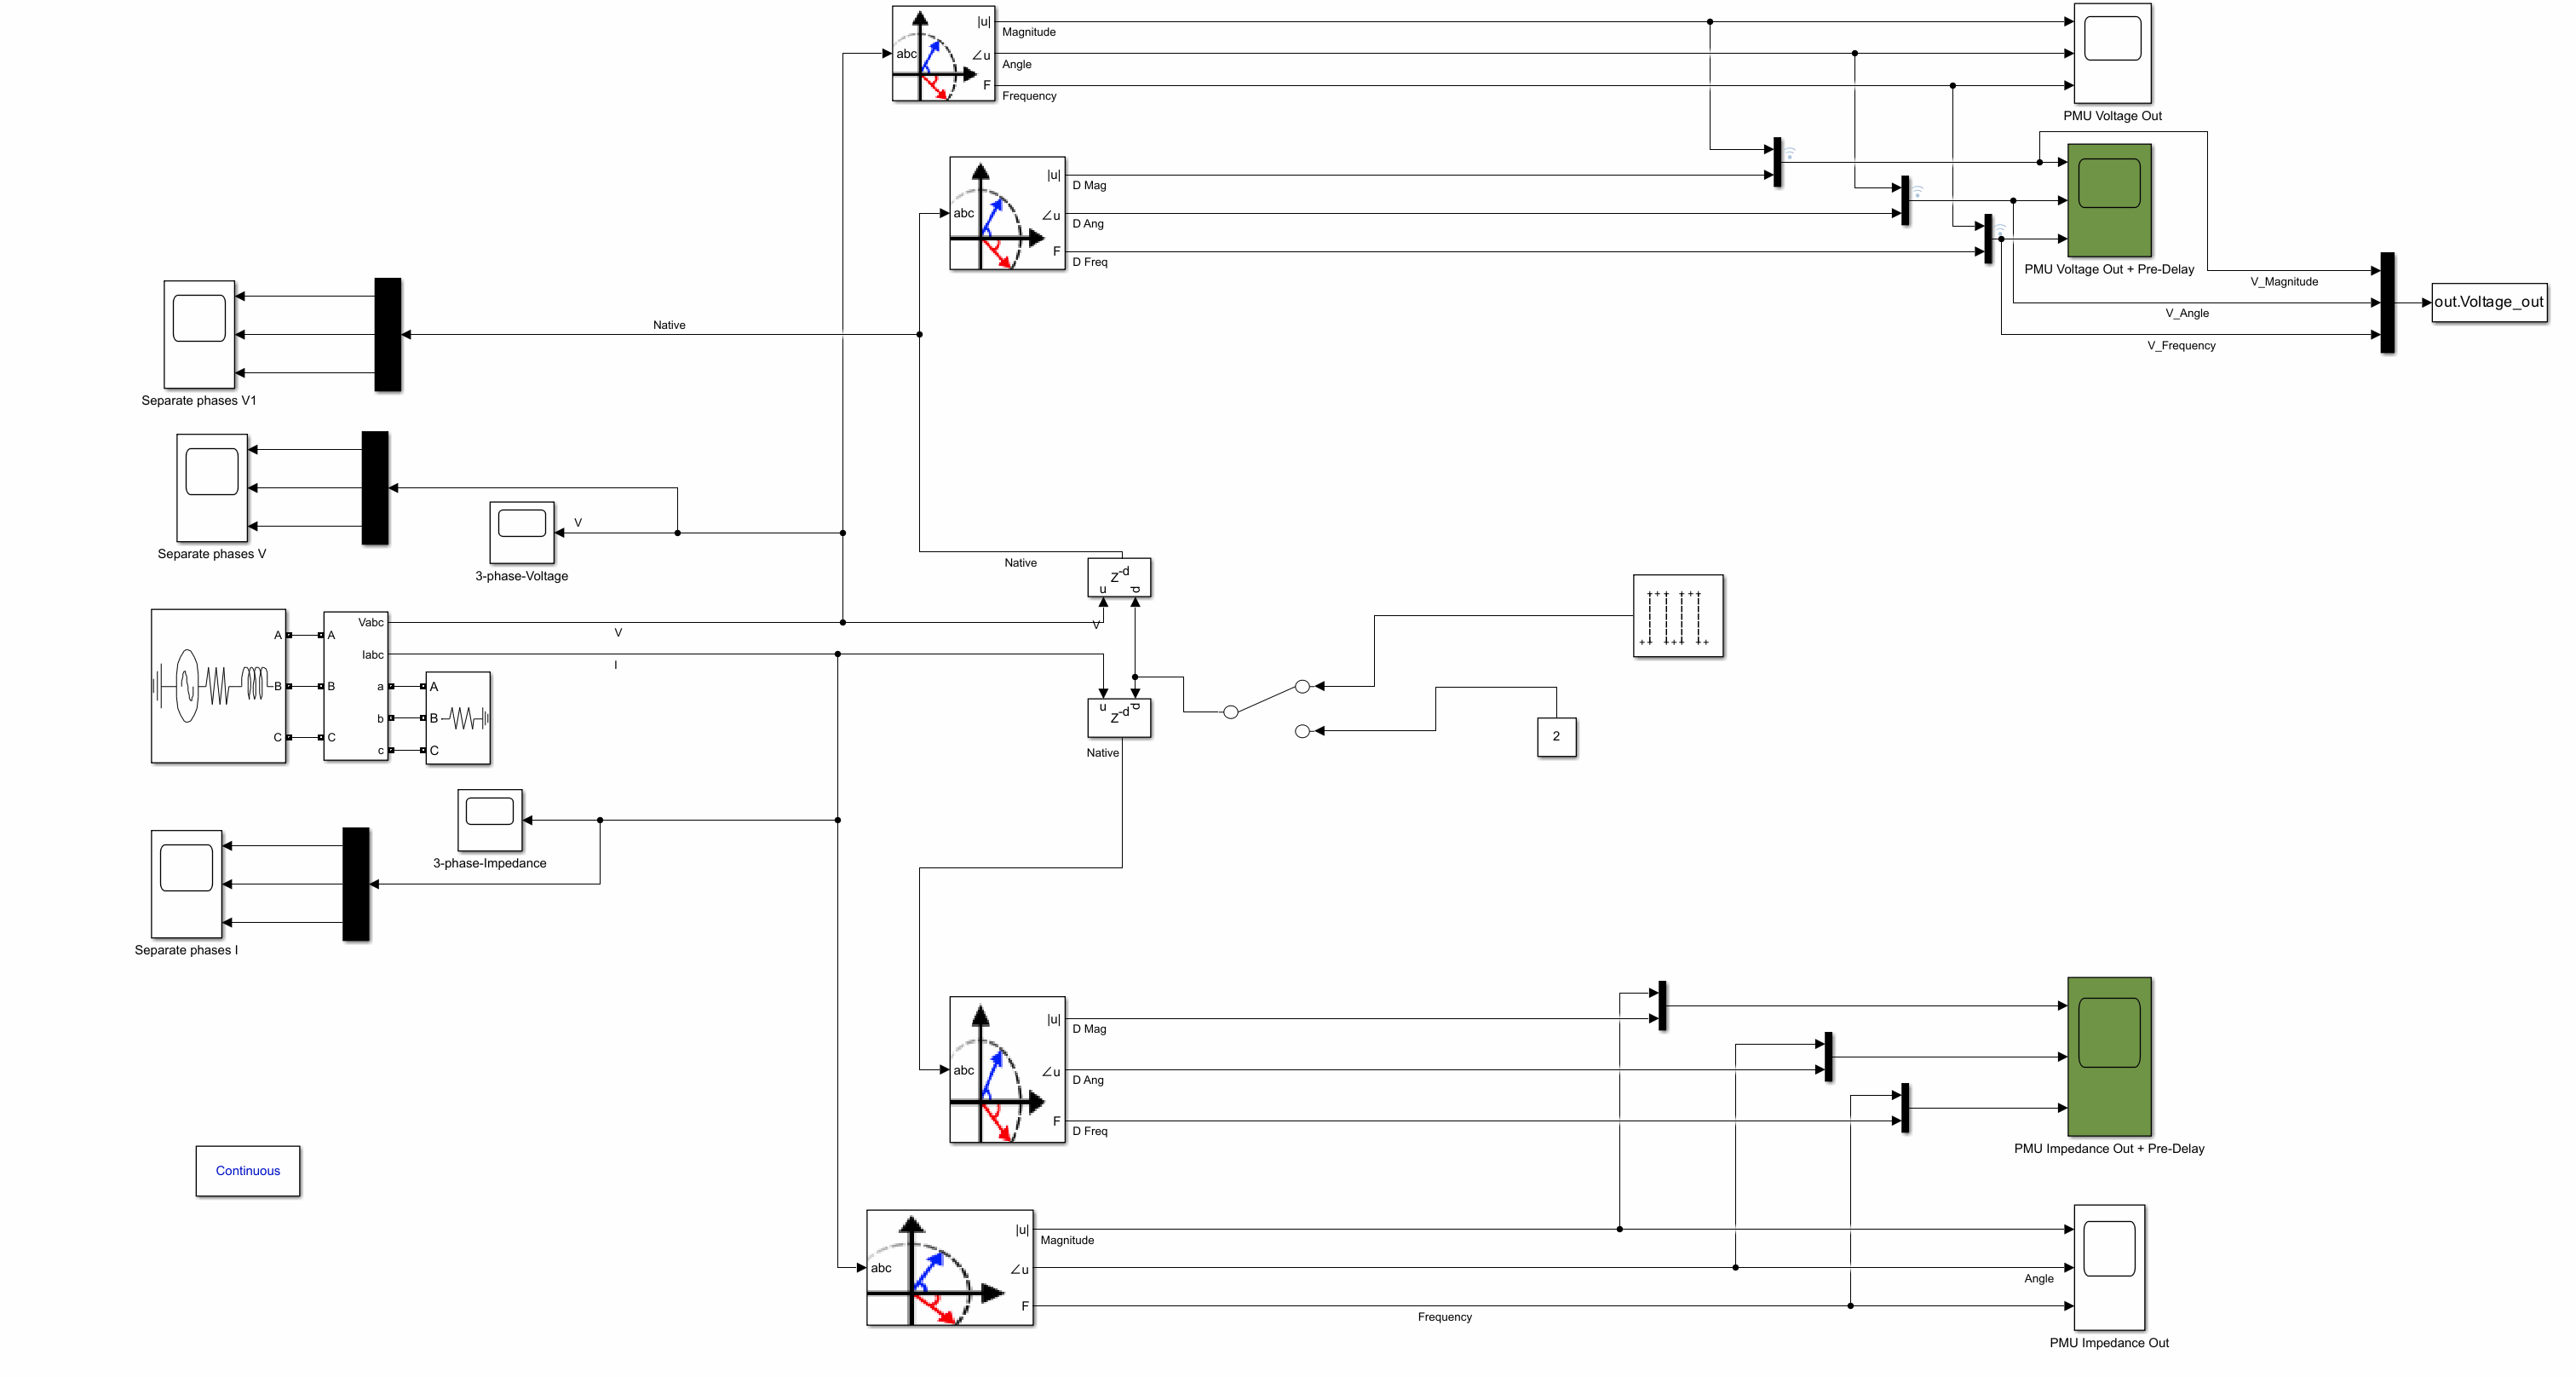
\includegraphics[width=\textwidth]{figures/SimPMU.png}
\caption[PmuSIM SIMULINK model]{A SIMULINK model for the simulation of PMU time delay attacks}

\end{figure}



\subsection{Experimental Procedure}
%\textbf{TO DO:} \textit{Describe experimental procedure, dependant on experiments and experimental environment selected.}.
In order to complete one iteration of the simulation, each step should be completed, as required.
\begin{enumerate}
    \item Start Matlab
    \item Open a MATLAB script, named \textbf{PMUsimScript.m}.
    \item Inspect and modify a selection of variables, and execute the script for each run. The script will produce:
    \begin{enumerate}
    \item Output data logged to workspace according to the model.
    \item For each variation, a numeric comparison, followed by a corresponding colored (Green/Red) similarity classification.
    \item One combined figure showing original and delayed signal, as well as one figure for each of the PMU components "Angle", "Frequency" and "Magnitude".
    \item The figures are stored as specified in the MATLAB script.
    \end{enumerate}
    \item Planned analysis is to be determined, using component output generated. 
\end{enumerate}
Assumptions: 
Focus on a few optional tolerance levels. One Option: Assume a similarity of 0.95 to be hardly detectable.  
\begin{itemize}
    \item Use the lowermost drawings appearing in each component output generated for graph comparisons.
    \item Visually inspect the green portion, indicating tolerable difference as well as any red portions.
    \item The graphs may provide indications on attack stealthiness, by no, (or minimal) red portions in the lower drawing. 
    \item Tolerance levels: $1\% (0.01)$, $5\% (0.05)$ and $10\% (0.1)$ For now $1\%$ is covered.
\end{itemize}

\begin{enumerate}
    \item The green portion of the line indicates signal similarity, indication periods with a low probability of attack detection.
    \item The red portion of the graph is to be interpreted as time periods where the attack detection risk is too high for the attack to remain stealthy for lengthy periods of time.

\end{enumerate}
\subsection{Definition of Experiments} \label{sec:ExpDef}

%As discussed in an \textbf{Earlier Chapter}, according to \textbf{SELECTED PAPERS}, the \acrshort{sg} \acrshort{se} systems analysed would detect attacks producing signal differences of various levels of similarity. %around $10-15\%$ similarity.





The experiments will focus on various levels of assumed detection thresholds.

My experiments will cover a selection of attack strategies for the selection of threshold levels of $1\%$, $5\%$ and $10\%$ similarities.

\begin{enumerate}
    \item \textbf{d\_mode = 1:} Delay on a constant level for the entire duration of the simulation. 
    \item \textbf{d\_mode = 2:} Square pulse signal: Starting off, turning constant-delay on,  before dropping to 0 before simulation end. 
    \item \textbf{d\_mode = 3:} Increasing to delay level specified, before dropping to 0 before simulation end. 
    %\item Increasing delay, drop to 0 before simulation end
\end{enumerate}

The current figures of chapter \ref{chap:Results} are produced by exposing the PMU to a variety of \textbf{d\_mode}s, as well as a selection of delay levels.



%The experiments, therefore, will focus on levels of delay of 0.1 to 0.15. For each level, the analysis will focus on various attack strategies, reaching the delay level in 1,2,3 and 4 steps, before keeping the delay for a total duration of  5 to 15 seconds.

%The experiments will be performed utilising \acrshort{pmu} simulation software, utilising available verification tools to ensure the compliance with established standards like the <--->
%The plan is to recreate experiments performed by <----> in a live environment, utilising  In order to test mitigation, mininet will be utilised

%Generate PMU data utilising simulators verified for compliance


%Utilise SADF \cite{SADF-framework} in MATLAB.

%Once again, in case you are running a causal study and an experiment, it is important to detail the experimental procedure.

%Explain, to the reader for example, what was the experimental task (what did the participants have to do?), the extraneous variables that were controlled (variables of the environment that could affect the cause and affect relationship).




\let\includegraphics-old\includegraphics

\let\includegraphics\includegraphicsold

\chapter{Results} \label{chap:Results}

%The results chapter should simply present the results of applying the methods presented in the method chapter without further ado. This chapter will typically contain many graphs, tables, etc. Sometimes it is natural to discuss the results as they are presented, combining them into a `Results and Discussion' chapter, but more often they are kept separate.\\ 

The following sections presents the results for each attack type, with subsections for the detection threshold levels selected, as defined in section \ref{sec:ExpDef} \\ 

Comments on the results are deferred to chapter \ref{chap:Discussions}
\newpage
\section{Ascending delay function}
\begin{figure}[hb]
 %   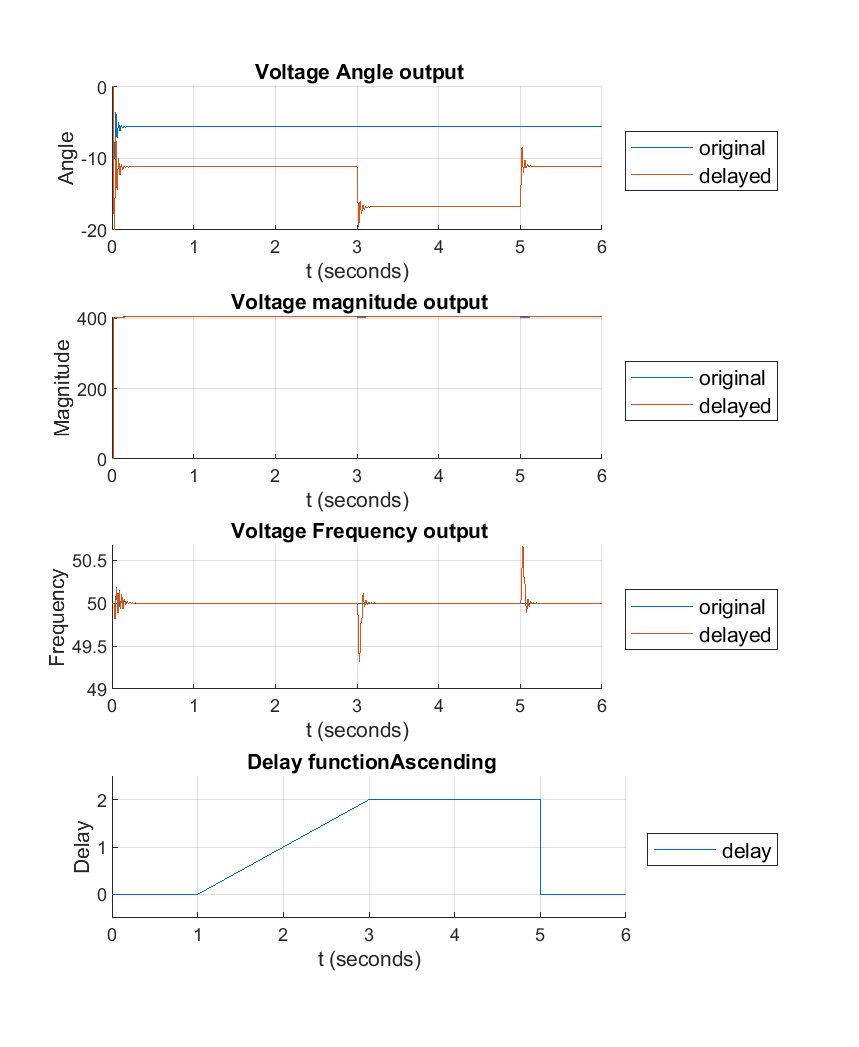
\includegraphics[trim=2 10 14 4, clip]{figures/v_AllFig-DelayOf_2-Ascending.png}    
    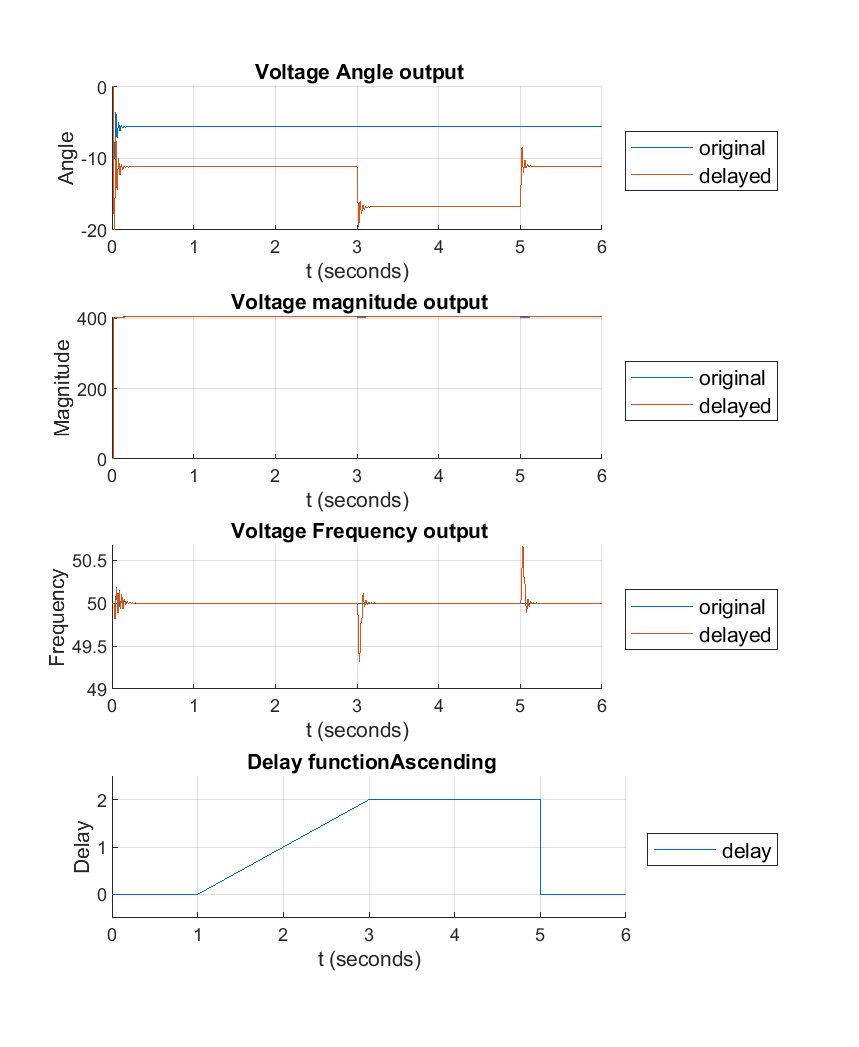
\includegraphics[width=0.95\textwidth]{figures/v_AllFig-DelayOf_2-Ascending.png}    
    \caption{Ascending delay combined output}
    \label{fig:simPMU-allfig}
\end{figure}


     \begin{figure}
        \caption{Component-wise output}
 
    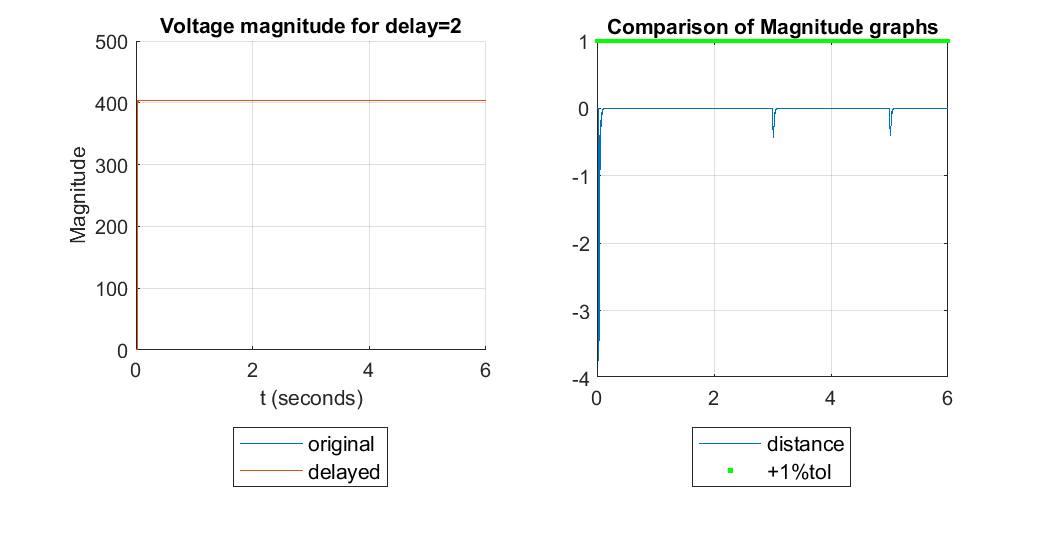
\includegraphics[width=0.95\textwidth]{figures/v_MagFig-DelayOf_2-Ascending.png}    
         %\caption{magnitude Output}
         \label{fig:AscMag}
   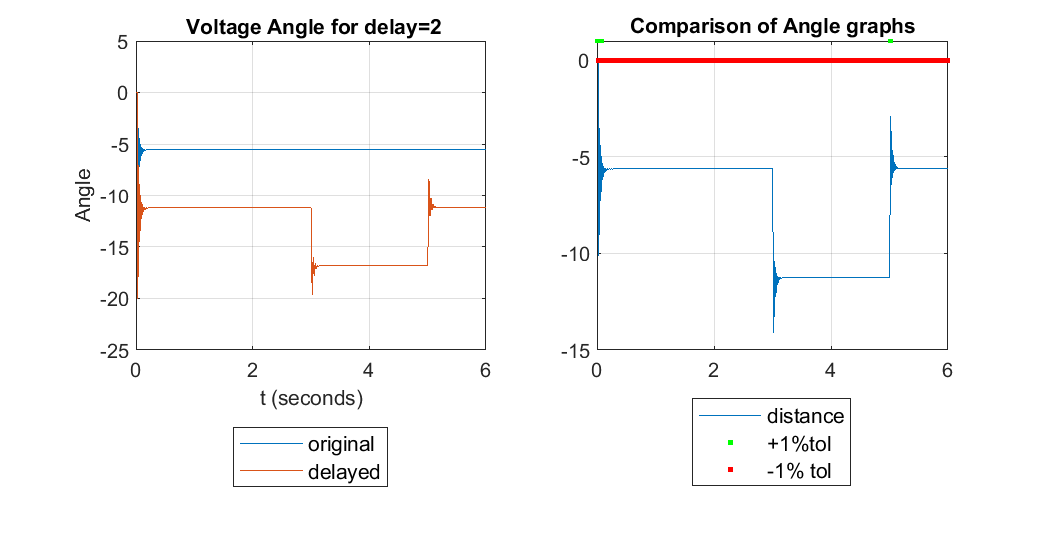
\includegraphics[width=0.95\textwidth]{figures/v_AngFig-DelayOf_2-Ascending.png}    
          %\caption{Angle Output}
         \label{fig:AscAng}
   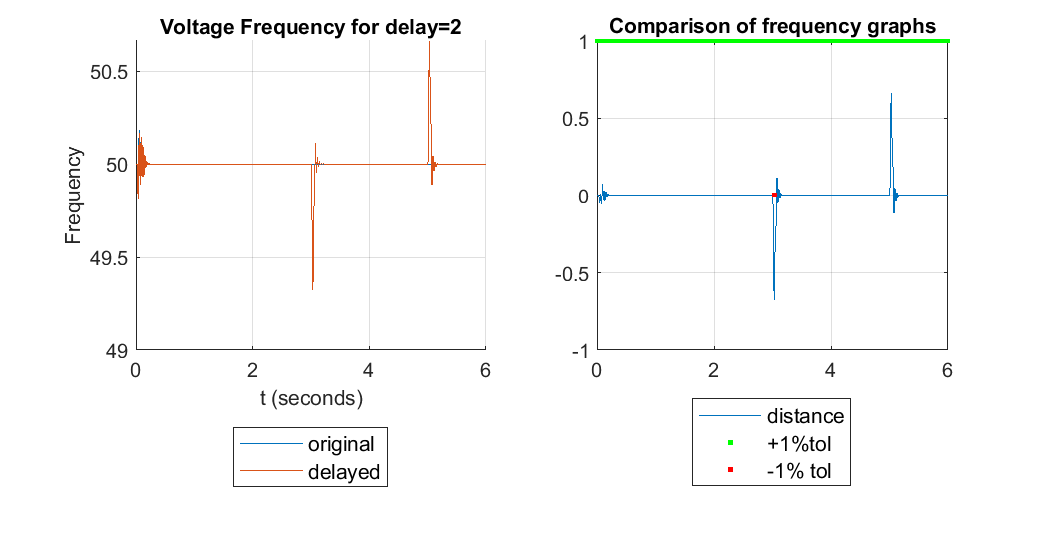
\includegraphics[width=0.95\textwidth]{figures/v_FreqFig-DelayOf_2-Ascending.png}    
         %\caption{frequency Output}
         \label{fig:AscFreq}
 
\end{figure}















%\section{off, on, off: abrupt}
%\subsection{Findings for a detection threshold level of 0.01}
%\subsection{Findings for a detection threshold level of 0.05}
%\subsection{Findings for a detection threshold level of 0.10}

%\section{increasing, on , decreasing: small steps}
%\subsection{Findings for a detection threshold level of 0.01}
%\subsection{Findings for a detection threshold level of 0.05}
%\subsection{Findings for a detection threshold level of 0.10}

%\section{increasing and continuous}
%\subsection{Findings for a detection threshold level of 0.01}
%\subsection{Findings for a detection threshold level of 0.05}
%\subsection{Findings for a detection threshold level of 0.10}

%\subsection{Findings for a detection threshold level of 0.01}
%\subsection{Findings for a detection threshold level of 0.05}
%\subsection{Findings for a detection threshold level of 0.10}
%\section{Findings for delay level 0.11}
%\section{Findings for delay level 0.12}
%\section{Findings for delay level 0.13}
%\section{Findings for delay level 0.14}
%\section{Findings for delay level 0.15}



\chapter{Discussion} \label{chap:Discussions}


%Here you should discuss all aspect of your thesis and project. How did the process work? Which choices did you make, and what did you learn from it? What were the pros and cons? What would you have done differently if you were to undertake the same project over again, both in terms of process and product? What are the societal consequences of your work?

\section{Introduction}


\subsection{Verification of model}

For verification purposes, results for the delay level of 0 is presented.  In this case, the original and delayed graphs should be identical.




\section{Probable answers to the Research Questions}

Discussion of results related to expected results, according to theoretical conclusions.




As previously stated in the introductory chapter, the main goal of my thesis is to answer the following RQ's: 

\begin{enumerate}
    \item Which effects do the time delay attack have on PMU output?
    \item For a selected similarity requirement, what delay level could be within similarity tolerance levels?
    \item What would characterise the optimal delay function, for the malicious actor to stay undetected?    
    %\item How might a \acrshort{sp} attack be mitigated?
    %\item Investigate the GPS spoofing vulnerability of the \acrshort{sg} monitoring and control system.
    %\item Investigate GPS Spoofing detection and mitigation techniques. 
    %\item Investigate how \acrfull{sdn} might be applicable to improve \acrshort{sg} Security
    %\item Investigate SDN-based SG \acrshort{dos} detection and mitigation potentials. 
    %\item 
\end{enumerate}

During this chapter, I will analyse the results of the previous chapter, searcing for answers to the research questions.

\subsection{Effects of time delay attack on PMU output}

\subsubsection{PMU Magnitude output effects}
A tendency of the \% tolerance graph to turn red at times of changes may be observed for most figures.

\subsubsection{PMU Angle output effects}

A tendency of the \% tolerance graph to stay red may be observed for most figures.


\subsubsection{PMU Frequency output effects}
In Figure \ref{fig:VoltageInstantDelayOne} for the Frequency output, however, the red part is visible for the lowest tolerance level only.
\subsection{Similarity Requirements}
In Figure \ref{fig:VoltageInstantDelayOne} (see above), for a similarity of 5\%, the attack detected  at level 1\% would stay undetected at level 5\%. 
\chapter{Conclusion}

%You definitely should use the \texttt{ntnuthesis} \LaTeX{} document class for your thesis.

\section{Introduction}
In order to answer the research questions
\section{Summary}

\section{Considerations related to further work}
\begin{itemize}
    \item One option for further work could be to investigate the options of the Power Source object included in the PowerSource subsystem, possibly redesigning the PowerSource with a more realistic Smart Grid Transmission system.
\item Another option could be to replace the PMUs of the Dual PMU subsytem, with different PMU implementations.
\end{itemize}


Those options are independent, and could be combined.





%\chapter{Power Grid  Security}


On of the implications of the transition from the \acrlong{pg} to the \acrlong{sg}, is the connection of  the traditionally closed and  proprietary energy distribution infrastructure to the Internet. 
Connecting the grid to the Internet  makes the grid available for monitoring and control purposes while exposing the grid to new threats, most notably the threats from external threat actors now able to attack the infrastructure from remote locations. 




\section{Classic Power Grid Security}

The Classical Power Grid consists of systems designed in order to provide a stable supply of electical power to a number of customers. As explained by \citeauthor{knapp2015industrial} in \cite{knapp2015industrial}, \acrshort{ics}s, like the \acrlong{pg}, has traditionally been airgapped systems, not designed with Cyber security in mind, including the continuous software and operating system updates so characteristic of any contemporary computer system. \\

The increased vulnerabilities to external threats observable as a consequence of connecting the grid to the Internet, has resulted in numerous activities related to securing the grid, wile reaping the substantial benefits of keeping the grid online. 



\subsection{Industrial Control System (ICS) Security}


Traditionally, the operational sites of any \acrfull{ics},  has been closed systems, not connected to public networks like the Internet. The \acrshort{pg}, and to some extent\footnote{The \acrshort{scada} subsystem of the \acrlong{sg} is part of the \acrshort{sg} \acrshort{wams} control system} even the \acrshort{sg}, utilises the \acrshort{scada} subsystem, for monitoring and control, 
The principle of "Security by Obscurity" has, as explained by  \citeauthor{humayed2017cyber}  in \cite{humayed2017cyber}, has been a dominant design principle for the traditional, offline, \acrlong{ics}.
As further explained  in \cite{humayed2017cyber}, most attacks on Industrial Control Systems, has been internal prior to 2001. Consequently, over the years following 2001, most of the attacks on \acrshort{ics} has been of external origin.





\subsection{Cyber Physical Systems security}

A \acrfull{cps} constitutes, as described in the previous chapter, of a physical production system, typically a \acrfull{ics} combined with a Cyber system connected the production system to public networks for monitoring and management purposes. As described by \citeauthor{humayed2017cyber} in \cite{humayed2017cyber}, the \acrshort{cps} may be of several types, amongst them the \acrshort{sg}.

The \acrshort{cps} constitutes a highly complex system,  combining physical production systems with systems connecting the physical systems to the outside world.\  

The authors of \cite{humayed2017cyber} provides some general characteristics of \acrshort{cps} security threats common to the various types of \acrshort{cps} identified:



\begin{itemize}
    \item 
    \item  
\end{itemize}




In addition, \figureautorefname{ }  \ref{fig:CP-Vulnerabilities-SG.png} presents vulnerabilities chrarcteristic of \acrshort{sg} \acrshort{ics}s:


\begin{figure}[ht]
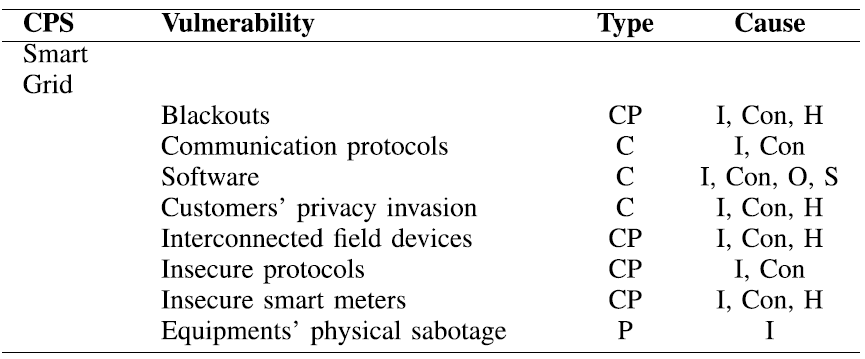
\includegraphics[width=\linewidth]{figures/CP-Vulnerabilities-SG.png}
\caption[\acrlong{cps} vulnerabilities for the \acrlong{sg}]{\acrlong{cps} vulnerabilities for the \acrlong{sg}, with causes. \cite[p. 1809]{humayed2017cyber}}
\label{fig:CP-Vulnerabilities-SG.png}
\end{figure}

As described in \citeauthor{humayed2017cyber}, "Type" and "Cause" are abbreviated as follows: Type classifications (C:CYBER, CP: CYBER-PHYSICAL, P: PHYSICAL, I: ISOLATION) and Causes (Con: CONNECTIVITY, O: OPENNESS, H: HETEROGENEITY,  S: MANY STAKEHOLDERS).






\section{Smart Grid  Security} 

\subsection{Smart Grid Security Requirements}
In order to protect the grid form new threat scenarios, a set of new security requirements needs to be defined in order to address the new situation. 
 
In \cite{Shapsough2015}, \citeauthor{Shapsough2015}  describes some information security concepts related to \acrlong{sg} security, defining the requirements in order to ensure the information security of the \acrshort{sg}. Thus, the \acrlong{sg} information security requirements might be summarised as follows:

\begin{itemize}
    \item \textbf{Availability} of the \acrlong{sg} is mandatory, as a violation of \acrlong{sg} availability implies a disruption of electricity. The immediate recovery from the lack of availability, is critical to the continued operation of a large number of services in a modern society.  
    \item \textbf{Integrity} violations in the \acrshort{sg} might affect power management, due to unauthorised modifications by illegitimate users. 
    \item \textbf{Confidentiality} violations will affect the privacy of users. Asides from the annoyance of privacy violations, power grid usage information might be indicative of empty buildings which could be a nice target for thieves. \item \textbf{Authentication} violations enables unauthorised access to private information, as well as \acrfull{sg} resources.
    \item \textbf{Authorisation} implements access control, preventing improper access to and management of \acrshort{sg} resources by unauthorised individuals.      \item \textbf{Non-Repudiation} violations enables individuals to deny being accessing or utilising \acrshort{sg} resources. Being able to track down actions of individual actors accessing \acrshort{sg} is vital due to the criticality of the \acrshort{sg}.
\end{itemize}


\section{Smart Grid Network Reliability and Security}

Two interrelated concepts are essential for the safe operation of the \acrshort{sg}:  
\begin{itemize}
    \item \acrlong{sg} \textbf{Network Reliability } which is important for the correct \acrshort{sg} operation, minimising the risk of \acrshort{sg} operational failures caused by \textbf{unintentional disruptive events} affecting \acrshort{sg} operations.
    
    \item \acrlong{sg} \textbf{Network Security}  which is important for the correct \acrshort{sg} operation, minimising the risk of \acrshort{sg} operational failures caused by \textbf{intentional malicious events}  affecting \acrshort{sg} operations.
\end{itemize}



\subsection{Smart Grid Network Reliability}

\subsection{Smart Grid Network Security}




    

\subsection{Synchrophasor  Protocol Threats}
Given the criticality of Time Synchronisation for the correct operation of the \acrshort{sg}, it is of vital importance to be aware of which threats imposes security risks related to the underlying Time Protocol. As explained by \citeauthor{mizrahi2014security} in \Cite{mizrahi2014security}, several attacker types could inflict a number of attacks on various time protocols. My introductory coverage of time protocol threats includes descriptions on attacker types and attack types, for reference purposes.








%\input{chapters/06-Simulation}
%\chapter{Using the Document Class}
\label{chap:usage}

\section{Thesis Setup and Language Selection}
\label{sec:setup}

The document class is initialized by issuing the \texttt{\textbackslash documentclass[]\{ntnuthesis\}} at the beginning of your \texttt{.tex} file. The thesis language should be given as an option. Currently British English (class option \texttt{[british]}), American English (class option \texttt{[american]}), Norwegian Bokmål (class option \texttt{[norsk]}) and Norwegian Nynorsk (class option \texttt{[nynorsk]}) are supported.\footnote{Disclaimer: this unfortunate naming of the Norwegian language options follows from the naming conventions of the \texttt{babel} package.}

There is also the \texttt{titlepage} class option that triggers the generation of a simple title page that can be used as a placeholder when writing the thesis. This option should be removed before handing in the thesis. Instead the official NTNU titlepage for the corresponding thesis type should be added as described on Innsida.\footnote{see \url{https://innsida.ntnu.no/wiki/-/wiki/English/Finalizing+the+bachelor+and+master+thesis} for bachelor and master, and \url{https://innsida.ntnu.no/wiki/-/wiki/English/Printing+your+thesis} for PhD.}

\section{Title, Author, and Date}

In the preample of the \texttt{.tex} file, the thesis title should be set with the \texttt{\textbackslash title\{\}} command. The title will appear on the titlepage as well as in the running header of the even numbered pages. If the title is too long for the header, you can use \texttt{\textbackslash shorttitle\{\}} to set a version for the header.

The authors should be listed with full names in the \texttt{\textbackslash author\{\}} command. If there are several authors, they should be separated with \texttt{\textbackslash and}, e.g., like this: \texttt{\textbackslash author\{Anne Andersen \textbackslash and Bjørn Bjørnsen\}}. For the running headers, you may want to use \texttt{\textbackslash shortauthor}, e.g. like this: \texttt{\textbackslash shortauthor\{A. Andersen and B. Bjørnsen\}} or even \texttt{\textbackslash shortauthor\{Andersen et al.\}}.

Use \texttt{\textbackslash date\{\}} to set the date of the document. It will only  appear on the temporary title page. To keep track of temporary versions, it can be a good idea to use \texttt{\textbackslash date\{\textbackslash today\}} while working on the thesis. You may also add copyright and licence information in this field.

\section{Page Layout}

The document class is designed to work with twosided printing. This means that all chapters start on odd (right hand) pages, and that blank pages are inserted where needed to make sure this happens. However, since the theses are very often read on displays, the margins are kept the same on even and odd pages in order to avoid that the page is jumping back and forth upon reading.

\section{Structuring Elements}

The standard \LaTeX{} elements for document structure are supported: chapter, section, and:

\subsection{This is a \texttt{\textbackslash subsection\{\}}}

Short subsection text here.

\subsubsection{This is a \texttt{\textbackslash subsubsection\{\}}}

Short subsubsection text here. 

\paragraph{This is a \texttt{\textbackslash paragraph\{\}}}

Short paragraph text here.

Chapters, sections, and subsections will be included in the table of contents, whereas the lower level structuring elements will not appear there. Don't use too many levels of headings; how many are appropriate, will depend on the size of the document. Also, don't use headings too frequently.

Make sure that the chapter and section headings are correctly capitalised depending on the language of the thesis, e.g., `\emph{Correct Capitalisation of Titles in English}' vs. `\emph{Korrekt staving av titler på norsk}'. 

Simple paragraphs are the lowest structuring elements and should be used the most. They are made by leaving one (or more) blank line(s) in the \texttt{.tex} file. In the typeset document they will appear indented and with no vertical space between them.

\section{Lists}

Numbered and unnumbered lists, i.e., the \texttt{enumerate} and \texttt{itemize} environments, are used just as in regular \LaTeX{}, but are typeset somewhat more densely and with other labels. Unnumbered list:
\begin{itemize}
    \item first item
    \item second item
    \begin{itemize}
        \item first subitem
        \item second subitem
        \begin{itemize}
            \item first subsubitem
            \item second subsubitem
        \end{itemize}
    \end{itemize}
    \item last item
\end{itemize}
Numbered list:
\begin{enumerate}
    \item first item
    \item second item
    \begin{enumerate}
        \item first subitem
        \item second subitem
        \begin{enumerate}
            \item first subsubitem
            \item second subsubitem
        \end{enumerate}
    \end{enumerate}
    \item last item
\end{enumerate}

For description lists, see usage in, e.g., \cref{sec:frontmatter}.

\section{Figures}

Figures are placed in the \texttt{figure} environment. An example is shown in \cref{fig:mapNTNU}. Figures are floats, hence they will float freely around in the document in accordance with standard \LaTeX{} behaviour. You may want to try to override \LaTeX{}'s default placement by using the \texttt{h} (here), \texttt{t} (top of page), \texttt{b} (bottom of page), and \texttt{p} (separate page) options in order of priority. If you provide an alternate (typically shorter) caption in square brackets, it will be used in the list of figures. Use \texttt{\textbackslash includegraphics[]\{\}} with options \texttt{scale} or \texttt{width} to include the graphics file. The caption should be placed \emph{below} the figure. If the caption consists of a single sentence fragment (incomplete sentence), it should not be punctuated. Given the shape and size of the figure, the figure caption can appear too close or too far from the figure. To deal with this, vertical space, either positive or negative, can be added before and/or after the caption command using the \texttt{\textbackslash vspace{}} command.

\begin{figure}[htbp]  % order of priority: h here, t top, b bottom, p page
  \centering
  \includegraphics[width=.5\textwidth]{figures/kart_student}
  \caption[Map of NTNU Campuses]{The map shows the three main campuses of NTNU.}
  \label{fig:mapNTNU}
\end{figure}

For figures compsed of several sub-figures, the \texttt{caption} and \texttt{subcaption} packages have been preloaded. See \cref{fig:subfig} with \cref{sfig:a,sfig:b} for an example. For more details on alignment etc., see the Overleaf documentation.\footnote{\url{https://www.overleaf.com/learn/latex/How_to_Write_a_Thesis_in_LaTeX_(Part_3):_Figures,_Subfigures_and_Tables}}

\begin{figure}
    \centering
    \begin{subfigure}[b]{.45\textwidth}
        \centering
        \includegraphics[width=\textwidth]{figures/kart_student.png}
        \caption{First sub-figure}
        \label{sfig:a}
    \end{subfigure}
    \hfill
    \begin{subfigure}[b]{.45\textwidth}
        \centering
        \includegraphics[width=\textwidth]{figures/kart_student.png}
        \caption{Second sub-figure}
        \label{sfig:b}
    \end{subfigure}
    \caption{A figure composed of two sub-figures. It has a long caption in order to demonstrate how that is typeset.}
    \label{fig:subfig}
\end{figure}

You can make nice graphs directly from data files using \texttt{gnuplot}, for an example, see \cref{fig:examplegnuplot}.

\begin{figure}[htbp]
  \centering
    \begin{gnuplot}[terminal=epslatex,terminaloptions={size 8cm,6cm color}]
        set xlabel "age" 
        set ylabel "IQ" 
        set key autotitle columnhead
        set title "age vs IQ"
        set yrange [0:160]
        set datafile separator ","
        plot "csvtables/ageiq.csv" using 1:2 with boxes 
    \end{gnuplot}
  \caption[An example of Integrated Graph]{This is a gnuplot graph read from a file. Also this figure has a long caption in order to demonstrate how that is typeset.}
  \label{fig:examplegnuplot}
\end{figure}

\section{Tables}

Tables are placed in the \texttt{table} environment. An example is given in \cref{tab:example1}. Like figures, tables float freely around in the document in accordance with standard \LaTeX{} behaviour. The table caption should be placed \emph{above} the table. If the caption consists of a single sentence fragment (incomplete sentence), it should not be punctuated.

\begin{table}
  \centering
  \caption{A simple, manually formatted example table}
  \label{tab:example1}
  \begin{tabular}{cc}
    \hline
    age  & IQ \\ 
    \hline
    10   & 110 \\
    20   & 120 \\
    30   & 145 \\
    40   & 120 \\
    50   & 100 \\
    \hline
  \end{tabular}
\end{table}

Tables can also be automatically generated from CSV files using the \texttt{simplecsv} and \texttt{booktab} packages. See \cref{tab:examplecsv} for an example.

\begin{table}[tbp]
  \centering
  \caption[A simple example table generated from a CSV file]{A simple example table generated from a CSV file using \texttt{simplecsv} and \texttt{booktab}}
  \label{tab:examplecsv}
  \csvautobooktabular{csvtables/ageiq.csv}
\end{table}

\section{Listings}

Code listings are included by means of the \texttt{listings} package. Code examples can be read from file or provided inline, and should be given a caption for cross referencing and for appearance in the list of code listings in the thesis frontmatter. If all your code examples are written in the same programming language, you can use, e.g., \texttt{\textbackslash lstset\{language=Python\}} to set the language once and for all. The code is set with the monospace font, and the font size is reduced to allow for code lines up to at least 80 characters without causing line breaks. Options for programming languages, line numbering etc. are provided. Unlike figures and tables, code listings are not floating objects, and will appear at the same position in the typeset document as in the \texttt{.tex} file. If the caption consists of a single sentence fragment (incomplete sentence), it should not be punctuated.

\lstinputlisting[
    caption={Python example from file},
    label=lst:pythonfile,
    language=Python
]{listings/example.py}

\lstinputlisting[%
    caption={C++ example from file},
    label=lst:cppfile,
    language=C++,
    numbers=left
]{listings/example.cc}

\begin{lstlisting}[
    caption={Python code in \LaTeX{} document},
    label=lst:pythondoc,
    language=Python]
import numpy as np
import matplotlib.pyplot as plt

x = np.linspace(0, 1)
y = np.sin(2 * np.pi * x)

plt.plot(x, y)
plt.show()
\end{lstlisting}

\begin{lstlisting}[
    caption={C++ code in \LaTeX{} document},
    label=lst:cppdoc,
    language=C++]
#include <iostream>
using namespace std;

int main() 
{
  cout << "Hello, World!" << endl;
  return 0;
}
\end{lstlisting}

\section{Equations}

Equations are typeset as normally in \LaTeX{}. It is common to consider equations part of the surrounding sentences, and include punctuation in the equations accordingly, e.g.,
\begin{equation}
    f(x) = \int_1^x \frac{1}{y}\,dy = \ln x\,.
    \label{eq:logarithm}
\end{equation}
For more advanced symbols like, e.g., $\mathbb{R}, \mathbb{Q}$, the \texttt{amssymb} package is preloaded, and for more advanced mathematical layout the \texttt{amsmath} behaviour is obtained through the \texttt{mathdesign} package. Confer the overleaf documentation for details.\footnote{\url{https://www.overleaf.com/learn/latex/Mathematical_expressions}}

\section{Fonts}

Bitstream Charter at 11pt with the corresponding Mathdesign math fonts have been selected as the main fonts for the thesis template. For code examples, the monospaced font should be used – for this, a scaled version of the DejaVuSansMono to match the main font is preselected. If you would like to use an accompanying sans serif font, the BeraSans has been made available. The standard \LaTeX{} font commands should be used to switch between fonts, e.g.,
\texttt{\textbackslash textit\{\}} \textit{for italics},
\texttt{\textbackslash textbf\{\}} \textbf{for bold face},
\texttt{\textbackslash texttt\{\}} \texttt{for mono spaced}, and
\texttt{\textbackslash textsf\{\}} \textsf{for sans serif}.
For generic \emph{emphasis}, \texttt{\textbackslash emph\{\}} should be applied.

\section{Cross References}
\label{sec:crossref}

For cross references, i.e., references within the document, the \texttt{\textbackslash cref\{\}} command provided byt the \texttt{cleveref} package should be used. Labels are inserted in the document in the standard \LaTeX{} manner. They are case sensitive, so, e.g., a label immediately after a section command refers to that section, while a label within, e.g., a table environment refers to the table. The \texttt{\textbackslash cref\{\}} command also generates the corresponding text. If the document is in English (class options \texttt{british} or \texttt{american}), the cross references are capitalised, whereas if it is in Norwegian (class options \texttt{norsk} or \texttt{nynorsk}), they are not. If you are writing in Norwegian, you should use \texttt{\textbackslash Cref\{\}} at the beginning of a sentence to ensure that the cross reference is correctly capitalised. For examples on usage, see \cref{sec:crossref} in \cref{chap:usage}, \cref{tab:example1}, \cref{fig:mapNTNU}, \cref{eq:logarithm}, \cref{lst:cppfile}, \cref{paper:scrutiny}, and \cref{app:additional}. \Cref{app:additional} at the beginning of a sentence.

The cross references are made into active hyperlinks in the resulting PDF document by the use of the \texttt{hyperref} package. The colour of the links is set to black for best appearance on print. This can easily be changed by the author by the use of the \texttt{\textbackslash hypersetup\{\}} command.

\section{Bibliography}

The bibliography is typset using the \texttt{biblatex} package with the \texttt{biber} backend. The default citation style is \texttt{numeric-comp}, and the default bibliography style is \texttt{numeric}. This produces a bibliography similar to, but not completely according to, the so-called Vancouver style. With this setup, a single \texttt{\textbackslash cite\{\}} command will give a number only~\cite{landes1951scrutiny}, and \texttt{\textbackslash textcite\{\}} will give author and number like this: \textcite{landes1951scrutiny}. If you would like to give the full reference of a paper within the thesis, e.g., in a list of included papers, use \texttt{\textbackslash fullcite\{\}} like this: \fullcite{landes1951scrutiny}.

\section{Included Papers}

If you are writing a compiled PhD thesis (and probably only then – see \cref{sec:compiledphd}), you will need to attach the papers containing the main contribution of the thesis. This can be done issuing the \texttt{paper} environment. It takes two arguments: (i) the PDF file, and (ii) a label for cross referencing. See \cref{paper:scrutiny} for an example.

\section{Appendices}

Additional material that does not fit in the main thesis but may still be relevant to share, e.g., raw data from experiments and surveys, code listings, additional plots, pre-project reports, project agreements, contracts, logs etc., can be put in appendices. Simply issue the command \texttt{\textbackslash appendix} in the main \texttt{.tex} file, and then the following chapters made by \texttt{\textbackslash chapter\{\}} become appendices. See \cref{app:additional} for an example.
%\chapter{Thesis Structure}

The structure of the thesis, i.e., which chapters and other document elements that should be included, depends on several factors such as the study level (bachelor, master, PhD), the type of project it describes (development, research, investigation, consulting), and the diversity (narrow, broad). Thus, there are no exact rules for how to do it, so whatever follows should be taken as guidelines only.

A thesis, like any book or report, can typically be divided into three parts: front matter, body matter, and back matter. Of these, the body matter is by far the most important one, and also the one that varies the most between thesis types.

\section{Front Matter}
\label{sec:frontmatter}

The front matter is everything that comes before the main part of the thesis. It is common to use roman page numbers for this part to indicate this. The minimum required front matter consists of a title page, abstract(s), and a table of contents. A more complete front matter, in a typical order, is as follows.

\begin{description}
    \item[Title page:] The title page should, at minimum, include the thesis title, authors and a date. A more complete title page would also include the name of the study programme, and possibly the thesis supervisor(s). See \cref{sec:setup}.
    \item[Abstracts:] The abstract should be an extremely condensed version of the thesis. Think one sentence with the main message from each of the chapters of the body matter as a starting point. \textcite{landes1951scrutiny} have given some very nice instructions on how to write a good abstract. A thesis from a Norwegian Univeristy should contain abstracts in both Norwegian and English irrespectively of the thesis language (typically with the thesis language coming first).
    \item[Dedication:] If you wish to dedicate the thesis to someone (increasingly common with increasing study level), you may add a separate page with a dedication here. Since a dedication is a personal statement, no template is given. Design it according to your preference.
    \item[Acknowledgements:] If there is someone who deserves a `thank you', you may add acknowledgements here. If so, make it an unnumbered chapter, i.e., \texttt{\textbackslash chapter*\{Acknowledgements\}}.
    \item[Table of contents:] A table of contents should always be present in a document at the size of a thesis. It is generated automatically using the \texttt{\textbackslash tableofcontents} command. The one generated by this document class also contains the front matter and unnumbered chapters.
    \item[List of figures:] If the thesis contains many figures that the reader might want to refer back to, a list of figures can be included here. It is generated using \texttt{\textbackslash listoffigures}.
    \item[List of tables:] If the thesis contains many tables that the reader might want to refer back to, a list of tables can be included here. It is generated using \texttt{\textbackslash listoftables}.
    \item[List of code listings:] If the thesis contains many code listings that the reader might want to refer back to, a list of code listings can be included here. It is generated using \texttt{\textbackslash lstlistoflistings}.
    \item[Other lists:] If there are other list you would like to include, this would be a good place. Examples could be lists of definitions, theorems, nomenclature, abbreviations, glossary etc. There are no standards for this, but many lists can be generated using the \texttt{description} environment (like, e.g., this list of possible front matter content) within a separate \texttt{\textbackslash chapter*\{\}}.
    \item[Preface or Foreword:] A preface or foreword is a good place to make other personal statements that do not fit whithin the body matter. This could be information about the circumstances of the thesis, your motivation for choosing it, or possibly information about an employer or an external company for which it has been written. Again, use, e.g., \texttt{\textbackslash chapter*\{Preface\}}.
\end{description}

\section{Body Matter}

The body matter consists of the main chapters of the thesis. It starts the Arabic page numbering with page~1. There is a great diversity in the structure chosen for different thesis types. Common to almost all is that the first chapter is an introduction, and that the last one is a conclusion followed by the bibliography.

\subsection{Development Project}
\label{sec:development}

For many bachelor and some master projects in computer science, the main task is to develop something, typically a software prototype, for an `employer' (e.g., an external company or a research group). A thesis describing such a project is typically structured as a software development report whith more or less the following chapters:

\begin{description}
    \item[Introduction:] The introduction of the thesis should take the reader all the way from the big picture and context of the project to the concrete task that has been solved in the thesis. A nice skeleton for a good introduction was given by \textcite{claerbout1991scrutiny}: \emph{review–claim–agenda}. In the review part, the background of the project is covered. This leads up to your claim, which is typically that some entity (software, device) or knowledge (research questions) is missing and sorely needed. The agenda part briefly summarises how your thesis contributes.
    \item[Requirements:] The requirements chapter should lead up to a concrete description of both the functional and non-functional requirements for whatever is to be developed at both a high level (use cases) and lower levels (low level use cases, requirements). If a classical waterfall development process is followed, this chapter is the product of the requirement phase. If a more agile model like, e.g., SCRUM is followed, the requirements will appear through the project as, e.g., the user stories developed in the sprint planning meetings.
    \item[Technical design:] The technical design chapter describes the big picture of the chosen solution. For a software development project, this would typically contain the system arcitechture (client-server, cloud, databases, networking, services etc.); both how it was solved, and, more importantly, why this architecture was chosen.
    \item[Development Process:] In this chapter, you should describe the process that was followed. It should cover the process model, why it was chosen, and how it was implemented, including tools for project management, documentation etc. Depending on how you write the other chapters, there may be good reasons to place this chapters somewhere else in the thesis.
    \item[Implementation:] Here you should describe the more technical details of the solution. Which tools were used (programming languages, libraries, IDEs, APIs, frameworks, etc.). It is a good idea to give some code examples. If class diagrams, database models etc. were not presented in the technical design chapter, they can be included here.
    \item[Deployment:] This chapter should describe how your solution can be deployed on the employer's system. It should include technical details on how to set it up, as well as discussions on choices made concerning scalability, maintenance, etc.
    \item[Testing and user feedback:] This chapter should describe how the system was tested during and after development. This would cover everything from unit testing to user testing; black-box vs. white-box; how it was done, what was learned from the testing, and what impact it had on the product and process.
    \item[Discussion:] Here you should discuss all aspect of your thesis and project. How did the process work? Which choices did you make, and what did you learn from it? What were the pros and cons? What would you have done differently if you were to undertake the same project over again, both in terms of process and product? What are the societal consequences of your work?
    \item[Conclusion:] The conclusion chapter is usually quite short – a paragraph or two – mainly summarising what was achieved in the project. It should answer the \emph{claim} part of the introduction. It should also say something about what comes next (`future work').
    \item[Bibliography:] The bibliography should be a list of quality-assured peer-reviewed published material that you have used throughout the work with your thesis. All items in the bibliography should be referenced in the text. The references should be correctly formatted depending on their type (book, journal article, conference publication, thesis etc.). If \texttt{biblatex} is correctly used as proposed by this template, the formatting will be taken care of automatically. The bibliography should not contain links to arbitrary dynamic web pages where the content is subject to change at any point of time. Such links, if necessary, should rather be included as footnotes throughout the document. The main point of the bibliography is to back up your claims with quality-assured material that future readers will actually be able to retrieve years ahead.
\end{description}

\subsection{Research Project}
\label{sec:resesarch}

For many master and some bachelor projects in computer science, the main task is to gain knew knowledge about something. A thesis describing such a project is typically structed as an extended form of a scientific paper, following the so-called IMRaD (Introduction, Method, Results, and Discussion) model:

\begin{description}
    \item[Introduction:] See \cref{sec:development}.
    \item[Background:] Research projects should always be based on previous research on the same and/or related topics. This should be described as a background to the thesis with adequate bibliographical references. If the material needed is too voluminous to fit nicely in the review part of the introduction, it can be presented in a separate background chapter.
    \item[Method:] The method chapter should describe in detail which activities you undertake to answer the research questions presented in the introduction, and why they were chosen. This includes detailed descriptions of experiments, surveys, computations, data analysis, statistical tests etc.
    \item[Results:] The results chapter should simply present the results of applying the methods presented in the method chapter without further ado. This chapter will typically contain many graphs, tables, etc. Sometimes it is natural to discuss the results as they are presented, combining them into a `Results and Discussion' chapter, but more often they are kept separate.
    \item[Discussion:] See \cref{sec:development}.
    \item[Conclusion:] See \cref{sec:development}.
    \item[Bibliography:] See \cref{sec:development}.
\end{description}

\subsection{Monograph PhD Thesis}
\label{sec:monograph}

Traditionally, it has been common to structure a PhD thesis as a single book – a \emph{monograph}. If the thesis is in the form of one single coherent research project, it can be structured along the lines of \cref{sec:resesarch}. However, for such a big work that a PhD thesis constitutes, the tasks undertaken are often more diverse, and thus more naturally split into several smaller research projects as follows:

\begin{description}
    \item[Introduction:] The introduction would serve the same purpose as for a smaller research project described in \cref{sec:development}, but would normally be somewhat more extensive. The \emph{agenda} part should inform the reader about the structure of the rest of the document, since this may vary significantly between theses.
    \item[Background:] Where as background chapters are not necessarily needed in smaller works, they are almost always need in PhD thesis. They may even be split into several chapters if there are significantly different topics to cover. See \cref{sec:resesarch}.
    \item[Main chapters:] Each main chapter can be structured more or less like a scientific paper. Depending on how much is contained in the introduction and background sections, the individual introduction and background sections can be significantly reduced or even omitted completely.
    \begin{itemize}
        \item (Introduction)
        \item (Background)
        \item Method
        \item Results
        \item Discussion
        \item Conclusion
    \end{itemize}
    \item[Discussion:] In addition to the discussions within each of the individual chapters, the contribution of the thesis \emph{as a whole} should be thoroughly discussed here.
    \item[Conclusion:] In addition to the conclusions of each of the individual chapters, the overall conclusion of the thesis, and how the different parts contribute to it, should be presented here. The conclusion should answer to the research questions set out in the main introduction. See also \cref{sec:development}.
    \item[Bibliography:] See \cref{sec:development}.
\end{description}

\subsection{Compiled PhD Thesis}
\label{sec:compiledphd}

Instead of writing up the PhD thesis as a monograph, compiled PhD theses (also known as stapler theses, sandwich theses, integrated theses, PhD by published work) consisting of reproductions of already published research papers are becoming increasingly common. At least some of the papers should already have been accepted for publication at the time of submission of the thesis, and thus have been through a real quality control by peer review.

\begin{description}
    \item[Introduction:] See \cref{sec:monograph}.
    \item[Background:] See \cref{sec:monograph}.
    \item[Main contributions:] This chapter should sum up \emph{and integrate} the contribution of the thesis as a whole. It should not merely be a listing of the abstracts of the individual papers – they are already available in the attached papers, and, as such, not needed here.
    \item[Discussion:] See \cref{sec:monograph}.
    \item[Conclusion:] See \cref{sec:monograph}.
    \item[Bibliography:] See \cref{sec:development}.
    \item[Paper I:] First included paper with main contributions. It can be included verbatim as a PDF. The publishers PDF should be used if the copyright permits it. This should be checked with the SHERPA/RoMEO database\footnote{\url{http://sherpa.ac.uk/romeo/index.php}} or with the publisher. Even when it is no general permission by the publisher, you may write and ask for one.
    \item[Paper II:] etc.
\end{description}

\section{Back Matter}

Material that does not fit elsewhere, but that you would still like to share with the readers, can be put in appendices. See \cref{app:additional}.











\chapter*{Bibliography}
\printbibliography[heading=none]
%\printbibliography

%% First paper

\begin{paper}{papers/landes1951scrutiny.pdf}{paper:scrutiny}
    Here, you may add a description of the paper, an illustration, or just give the bibliographic reference:
    \begin{quote}
        \fullcite{landes1951scrutiny}
    \end{quote}
    Or you may leave it empty, if you like.
\end{paper}

% Second paper etc.




\subsubsection{Traditional networking}
Traditional enterprise-class computer networks consists of a number of proprietary black-boxes, like branded\footnote{For instance Cisco, Catalyst and Juniper} routers and switches, consisting of data forwarding hardware network ports,controlled by a proprietary operating system. 

\begin{itemize}
\item{Vulnerable to (D)DoS} Traditional networks are vulnerable to \acrfull{ddos} attacks. \\

\item{Hard to manage} As each brand of network devices has its own proprietary management software, the flexibilty 
\end{itemize}

\begin{itemize}
\item cyber vulnerability assessment
\item redundant controllers

\item DDoS mitigation survey \cite{hameed2018sdn}
\item compares SDN controllers, recommending OpenDaylight\cite{arbettu2016security}.  \fullcite{arbettu2016security} 


\item traffic load balancing\cite{ejaz2019traffic} \\ \fullcite{ejaz2019traffic}

\end{itemize}



\subsubsection{Network Function Virtualisation}

Network Function Virtualisation (NFV) 




As part of the process of implementing the \acrshort{sg}, a thorough analysis of the security of the underlying network infrastructure is mandatory. 
In \cite{Shapsough2015},Shapsough et. al. discusses the cyber security of the \acrshort{sg}, related to various security requirements, including availability.The consequence of a successful \acrshort{dos} attack is a loss of electricity, which could inflict a serious impact on the modern society.

 %\fullcite{Shapsough2015}

%\acrfull{dos} attacks are identified as the most common threat to the \acrshort{sg}.


\begin{table}[ht]
\centering
\begin{tabular}{|c|l| p{8.5cm}| }
\hline
&Domain &Roles/Services in the Domain \\ \hline
 1&Customer &The end users of electricity. May also generate, store, and manage the
use of energy. Traditionally, three customer types are discussed, each
with its own domain: residential, commercial, and industrial. \\ \hline
 2&Markets&The operators and participants in electricity markets. \\\hline
 3&Service Provider &The organizations providing services to electrical customers and to
 utilities. \\\hline
 4&Operations & The managers of the movement of electricity. \\ \hline
 5&Generation &The generators of electricity. May also store energy for later
distribution. This domain includes traditional generation sources
(traditionally referred to as generation) and distributed energy
resources (DER). At a logical level, “generation” includes coal,
nuclear, and large-scale hydro generation usually attached to
transmission. DER (at a logical level) is associated with customer-
and distribution-domain-provided generation and storage, and with
service-provider-aggregated energy resources.\\ \hline
 6 & Transmission & The carriers of bulk electricity over long distances. May also store
and generate electricity. \\ \hline
 7 &Distribution &The distributors of electricity to and from customers. May also store
and generate electricity. \\
\hline
\end{tabular}
\caption{Table 5-1. Domains and Roles/Services in the\acrlong{sg} Conceptual Model}
\label{tab:SmartGRID-Roles-of-domains}
\end{table}







%The \acrshort{scada} system of the traditional \acrshort{sg} is expanded into the \acrfull{wams} system.




%\appendix
%\chapter{The project agreement}
\label{app:projectAgreement}

Additional material that does not fit in the main thesis but may still be relevant to share, e.g., raw data from experiments and surveys, code listings, additional plots, pre-project reports, project agreements, contracts, logs etc., can be put in appendices. Simply issue the command \texttt{\textbackslash appendix} in the main \texttt{.tex} file, and make one chapter per appendix.

If the appendix is in the form of a ready-made PDF file, it should be supported by a small descriptive text, and included using the \texttt{pdfpages} package. To illustrate how it works, a standard project agreement (for the IE faculty at NTNU in Gjøvik) is attached here. You would probably want the included PDF file to begin on an odd (right hand) page, which is achieved by using the \texttt{\textbackslash cleardoublepage} command immediately before the \texttt{\textbackslash includepdf[]\{\}} command. Use the option \texttt{[pages=-]} to include all pages of the PDF document, or, e.g., \texttt{[pages=2-4]} to include only the given page range.

\cleardoublepage
\includepdf[pages=-]{appendices/NTNUProsjektavtale.pdf}



%





  

\chapter[Smart Grid TSA Detection]{Smart Grid Time Synchronisation Attack Detection}





In order to cover the topic of \acrfull{tsa}s,  a general description of \acrshort{tsa} countermeasures, like detection and mitigation will be presented, before a number of case studies are presented and investigated.  


\section{Description}

   

\textbf{TO DO}

\textit{A description of the papers will be performed, focusing on case studies showing evidence of methods and techniques used for detection.}  \\ 


Some suggestions on relevant papers are:

    \begin{itemize}
    
    % Time synchronizationattack in smart grid: Impact and analysis
    \item  \cite{ZhangTimeSync2013}  \fullcite{ZhangTimeSync2013}
    
    % Vulnerability analysis of smart grids to gps spoofing
    \item  \cite{risbud2018vulnerability} \fullcite{risbud2018vulnerability}

    % Spatio-temporal characterization of synchrophasor data against spoofing attacks insmart grids
    \item  \cite{cui2019spatio}  \fullcite{cui2019spatio}

    % Vulnerab-ility of synchrophasor-based wampac applications’ to time synchronizationspoofing
    \item  \cite{almas2017vulnerability} \fullcite{almas2017vulnerability}
    
    % A gps spoofingresilient wams for smart grid
    \item  \cite{garofalo2013gps} \fullcite{garofalo2013gps}

    % Spoofing resilient state estimation forthe power grid using an extended kalman filter
    \item  \cite{chauhan2021spoofing} \fullcite{chauhan2021spoofing}

    % Multi-view con-volutional neural network for data spoofing cyber-attack detection in dis-tribution synchrophasors
    \item  \cite{qiu2020multi}  \fullcite{qiu2020multi}

    % A multi-layer perceptron neural network tomitigate the interference of time synchronization attacks in stationary gps receivers
    \item  \cite{orouji2021multi}  \fullcite{orouji2021multi}


    % Gps spoofing detection forthe power grid network using a multireceiver hierarchical framework archi-tecture
    \item  \cite{mina2019gps}  \fullcite{mina2019gps}

    % Precision time protocol attack strategiesand their resistance to existing security extensions
    \item  \cite{alghamdi2021precision} \fullcite{alghamdi2021precision}



    \end{itemize}
    

\section{Examples}


\textbf{TO DO:}
\textit{Describe examples of Smart Grid Time Synchronisation attack detection, found in the papers selected. }\\ 


%
\chapter[Smart Grid TSA Mitigation]{Smart Grid Time Synchronisation  Attack Mitigation}

\section{Description}

    
\textbf{TO DO}

\textit{A description of the papers will be performed, focusing on case studies showing evidence of methods and techniques used for mitigation.}  \\ 



Some suggestions on relevant papers are:

    \begin{itemize}
    
    % Time synchronizationattack in smart grid: Impact and analysis
    \item  \cite{ZhangTimeSync2013}  \fullcite{ZhangTimeSync2013}
    
    % Vulnerability analysis of smart grids to gps spoofing
    \item  \cite{risbud2018vulnerability} \fullcite{risbud2018vulnerability}

    % Spatio-temporal characterization of synchrophasor data against spoofing attacks insmart grids
    \item  \cite{cui2019spatio}  \fullcite{cui2019spatio}

    % Vulnerab-ility of synchrophasor-based wampac applications’ to time synchronizationspoofing
    \item  \cite{almas2017vulnerability} \fullcite{almas2017vulnerability}
    
    % A gps spoofingresilient wams for smart grid
    \item  \cite{garofalo2013gps} \fullcite{garofalo2013gps}

    % Spoofing resilient state estimation forthe power grid using an extended kalman filter
    \item  \cite{chauhan2021spoofing} \fullcite{chauhan2021spoofing}

    % Multi-view con-volutional neural network for data spoofing cyber-attack detection in dis-tribution synchrophasors
    \item  \cite{qiu2020multi}  \fullcite{qiu2020multi}

    % A multi-layer perceptron neural network tomitigate the interference of time synchronization attacks in stationary gps receivers
    \item  \cite{orouji2021multi}  \fullcite{orouji2021multi}


    % Gps spoofing detection forthe power grid network using a multireceiver hierarchical framework archi-tecture
    \item  \cite{mina2019gps}  \fullcite{mina2019gps}

    % Precision time protocol attack strategiesand their resistance to existing security extensions
    \item  \cite{alghamdi2021precision} \fullcite{alghamdi2021precision}



    \end{itemize}
      



\section{Examples}

\textbf{TO DO:}
\textit{Describe examples of Smart Grid Time Synchronisation attack mitigation, found in the papers selected.} \\ 


%\input{chapters/06-DDoS-Attacks}


\end{document}